% Options for packages loaded elsewhere
\PassOptionsToPackage{unicode}{hyperref}
\PassOptionsToPackage{hyphens}{url}

\documentclass[12pt,oneside]{book}
\usepackage{lmodern}
\usepackage[top=60pt,bottom=60pt,left=40pt,right=40pt]{geometry}
\usepackage{amssymb,amsmath}
\usepackage{ifxetex,ifluatex}
\usepackage{titlesec}
\ifnum 0\ifxetex 1\fi\ifluatex 1\fi=0 % if pdftex
  \usepackage[T1]{fontenc}
  \usepackage[utf8]{inputenc}
  \usepackage{textcomp} % provide euro and other symbols
\else % if luatex or xetex
  \usepackage{unicode-math}
  \defaultfontfeatures{Scale=MatchLowercase}
  \defaultfontfeatures[\rmfamily]{Ligatures=TeX,Scale=1}
\fi
% Use upquote if available, for straight quotes in verbatim environments
\IfFileExists{upquote.sty}{\usepackage{upquote}}{}
\IfFileExists{microtype.sty}{% use microtype if available
  \usepackage[]{microtype}
  \UseMicrotypeSet[protrusion]{basicmath} % disable protrusion for tt fonts
}{}
\makeatletter
\@ifundefined{KOMAClassName}{% if non-KOMA class
  \IfFileExists{parskip.sty}{%
    \usepackage{parskip}
  }{% else
    \setlength{\parindent}{0pt}
    \setlength{\parskip}{6pt plus 2pt minus 1pt}}
}{% if KOMA class
  \KOMAoptions{parskip=half}}
\makeatother
\usepackage{xcolor}
\IfFileExists{xurl.sty}{\usepackage{xurl}}{} % add URL line breaks if available
\IfFileExists{bookmark.sty}{\usepackage{bookmark}}{\usepackage{hyperref}}
\hypersetup{
  pdftitle={Rigs of Rods Manual},
  hidelinks}
\urlstyle{same} % disable monospaced font for URLs
\usepackage{graphicx}
\makeatletter
\def\maxwidth{\ifdim\Gin@nat@width>\linewidth\linewidth\else\Gin@nat@width\fi}
\def\maxheight{\ifdim\Gin@nat@height>\textheight\textheight\else\Gin@nat@height\fi}
\makeatother
% Scale images if necessary, so that they will not overflow the page
% margins by default, and it is still possible to overwrite the defaults
% using explicit options in \includegraphics[width, height, ...]{}
\setkeys{Gin}{width=\maxwidth,height=\maxheight,keepaspectratio}
% Set default figure placement to htbp
\makeatletter
\def\fps@figure{htbp}
\makeatother
\setlength{\emergencystretch}{3em} % prevent overfull lines
\providecommand{\tightlist}{%
  \setlength{\itemsep}{0pt}\setlength{\parskip}{0pt}}
\setcounter{secnumdepth}{-\maxdimen} % remove section numbering

%\titleformat{\chapter}[display]{\normalfont\huge\bfseries}{\chaptertitlename\ \thechapter}{20pt}{\Huge}   
%\titlespacing*{\chapter}{0pt}{-50pt}{0pt}

%\titlespacing{\chapter}{0.3pt}{0.3pt}{0.3pt}
%\titleformat{\chapter}[block]{\bfseries\Large}{\chaptertitle}{0.5em}{\Large\bfseries\filcenter}
%\titleformat{\chapter}{}{}{0pt}{\Huge\bfseries}

\title{Rigs of Rods Manual}

\begin{document}
\maketitle

\tableofcontents
\hypertarget{Beginners-Guide}{%
\chapter{Beginner's Guide}\label{Beginners-Guide}}

\hypertarget{introduction}{%
\section{Introduction}\label{introduction}}

\begin{quote}
Rigs of Rods (RoR) is a free/libre soft-body physics simulator mainly
targeted at simulating vehicle physics. The soft-body physics system is
based on mass-spring-damper theory.
\end{quote}

This page will help you learn the basics of Rigs of Rods, from
installing to playing multiplayer.

\hypertarget{first-run}{%
\section{First Run}\label{first-run}}

When launching RoR for the first time, the user directory will be
created. On Windows this is located at
\texttt{Documents\textbackslash{}Rigs\ of\ Rods\ 0.4} or at
\texttt{\textasciitilde{}/.rigsofrods} on Linux. This is where
configuration files, logs, and mods are stored.

The game should open in a small window:  

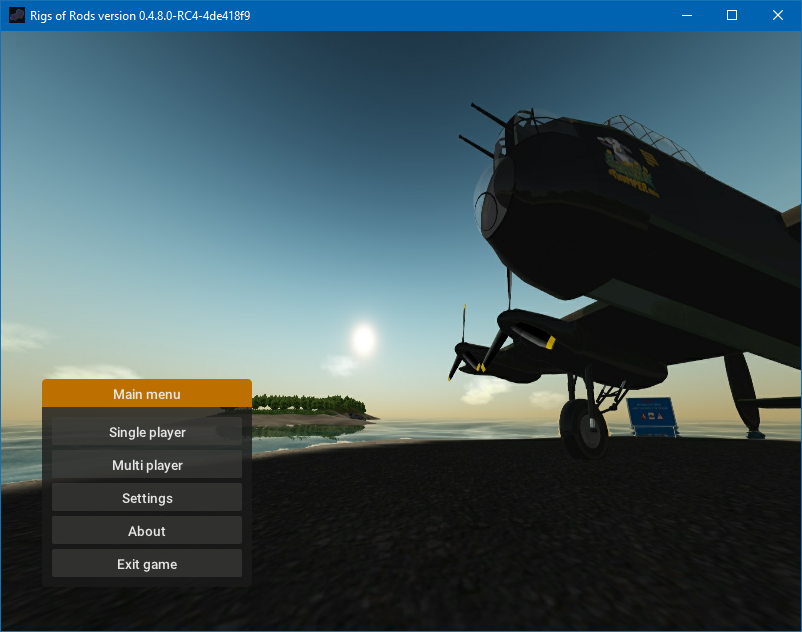
\includegraphics{images/bg-firstrun1.png}

Before playing, you should first change your settings. Begin by clicking
\texttt{Settings}.

First, make sure the rendering system is set to
\texttt{Direct3D9\ Rendering\ Subsystem}. If it's set to
\texttt{OpenGL\ Rendering\ Subsystem}, change it.

If you're running Linux, ignore this as DirectX is not available.

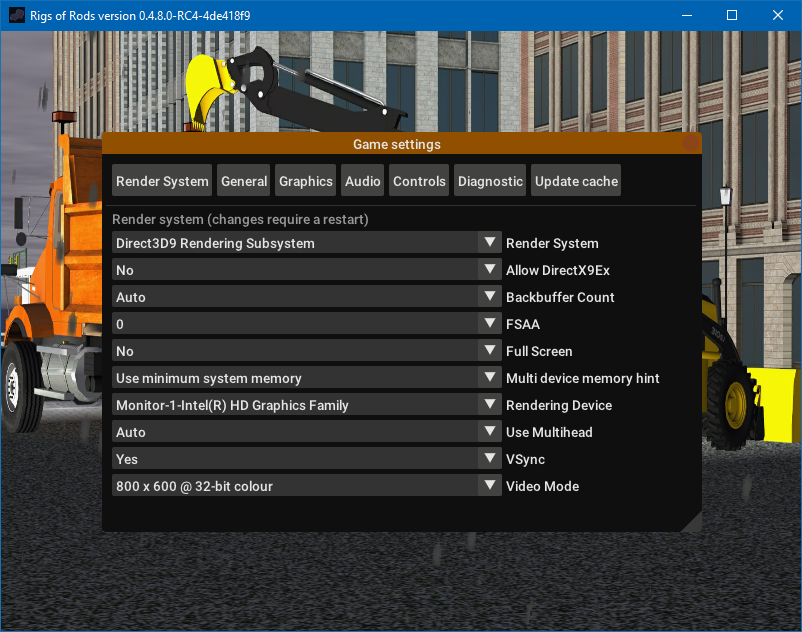
\includegraphics{images/bg-firstrun2.png}

Now select \texttt{Video\ Mode} and change it to your monitor's native
resolution then restart the game to apply your changes.


\includegraphics{images/bg-firstrun3.png}

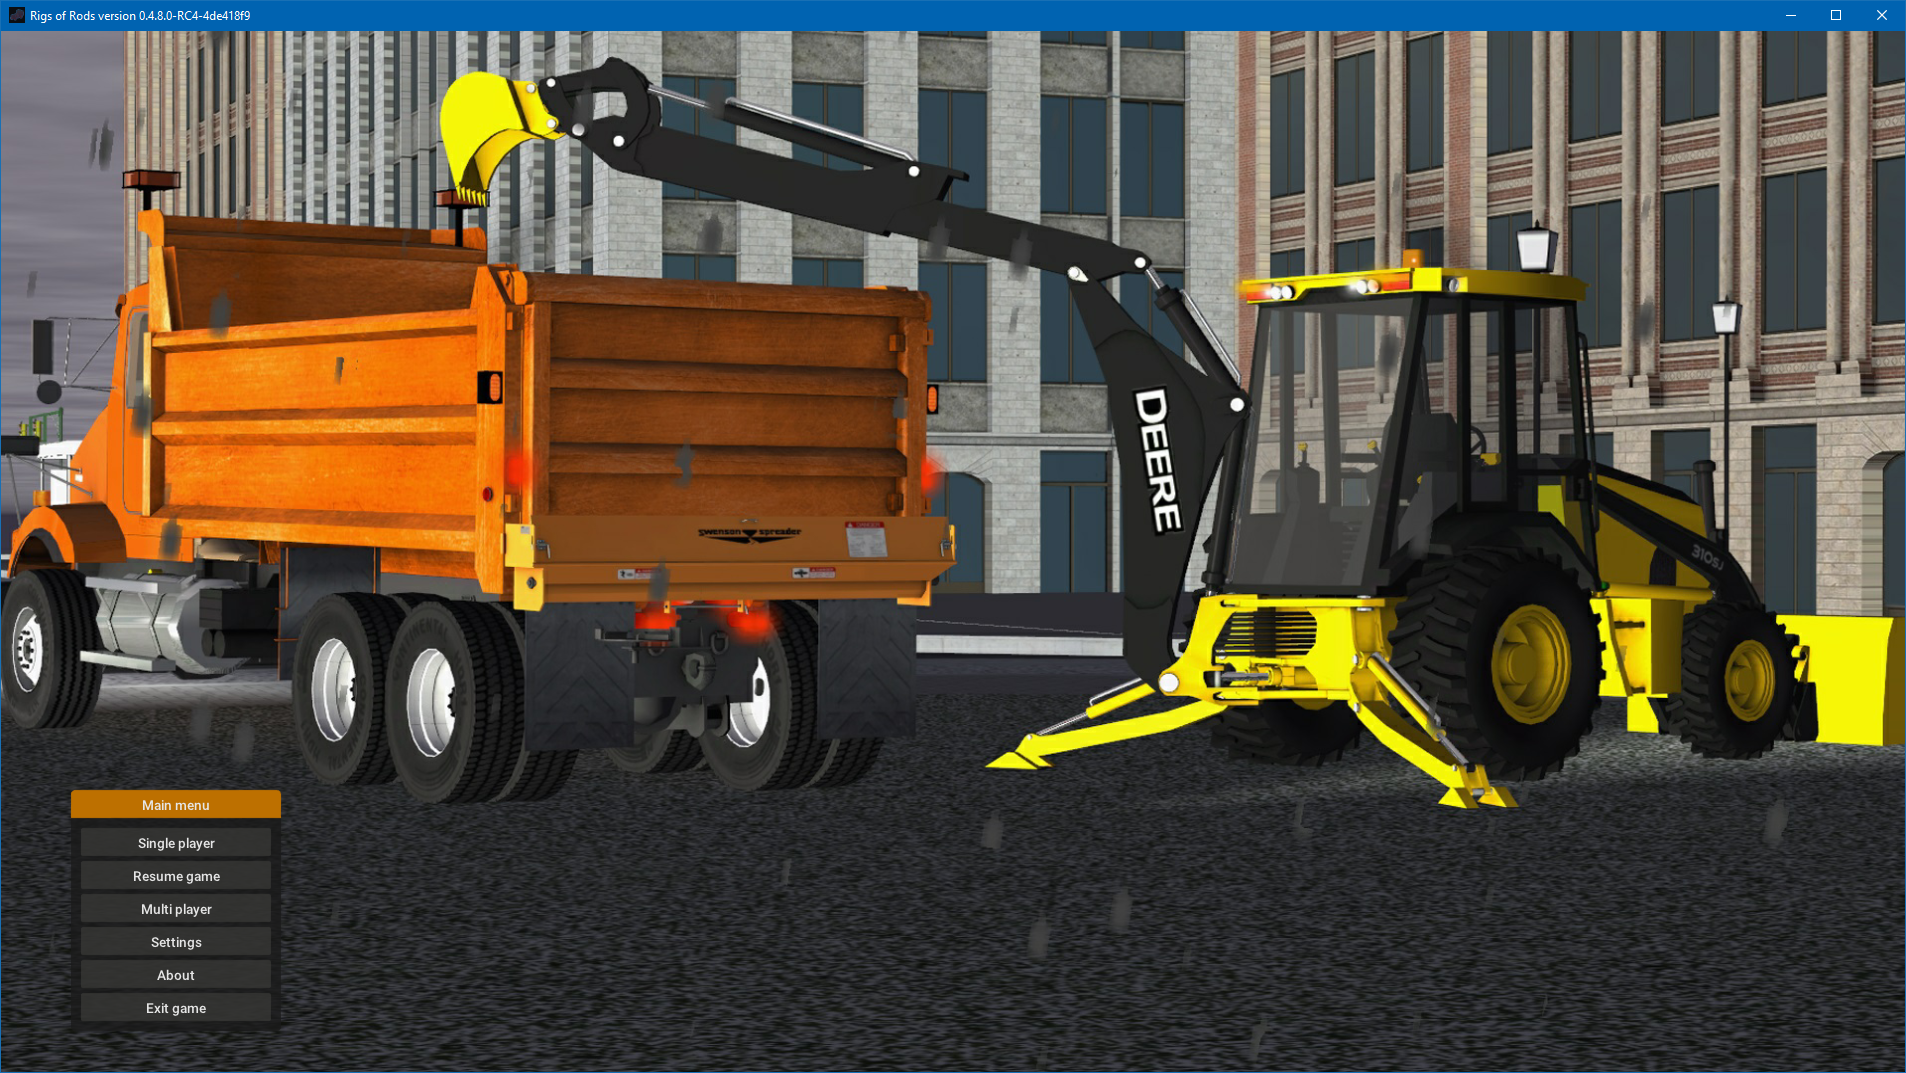
\includegraphics{images/bg-firstrun4.png}

Click \texttt{Settings} again, then click the \texttt{Graphics} tab.

The following settings should be fine for most people, but feel free to
adjust them to fit your liking.

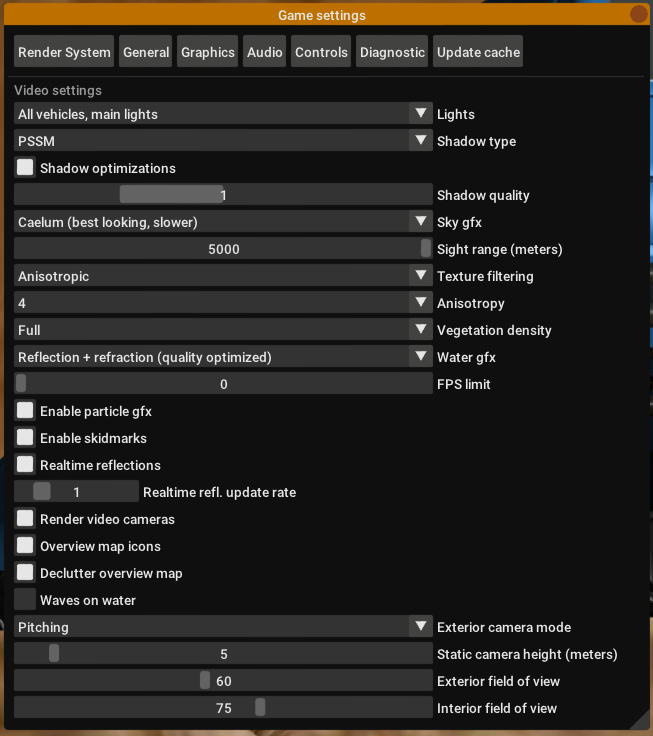
\includegraphics{images/bg-firstrun5.png}

Then click the \texttt{Audio} tab and set the volume. Due to a bug in
RC4, it is muted by default.

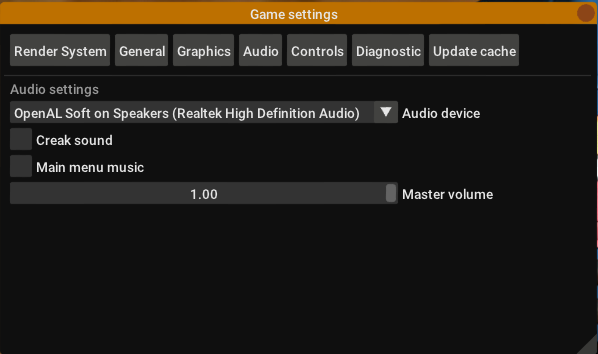
\includegraphics{images/bg-firstrun6.png}

Once you're finished, restart the game again.

Now you're ready to begin playing. Start by clicking
\texttt{Single\ player} to open the terrain selector.

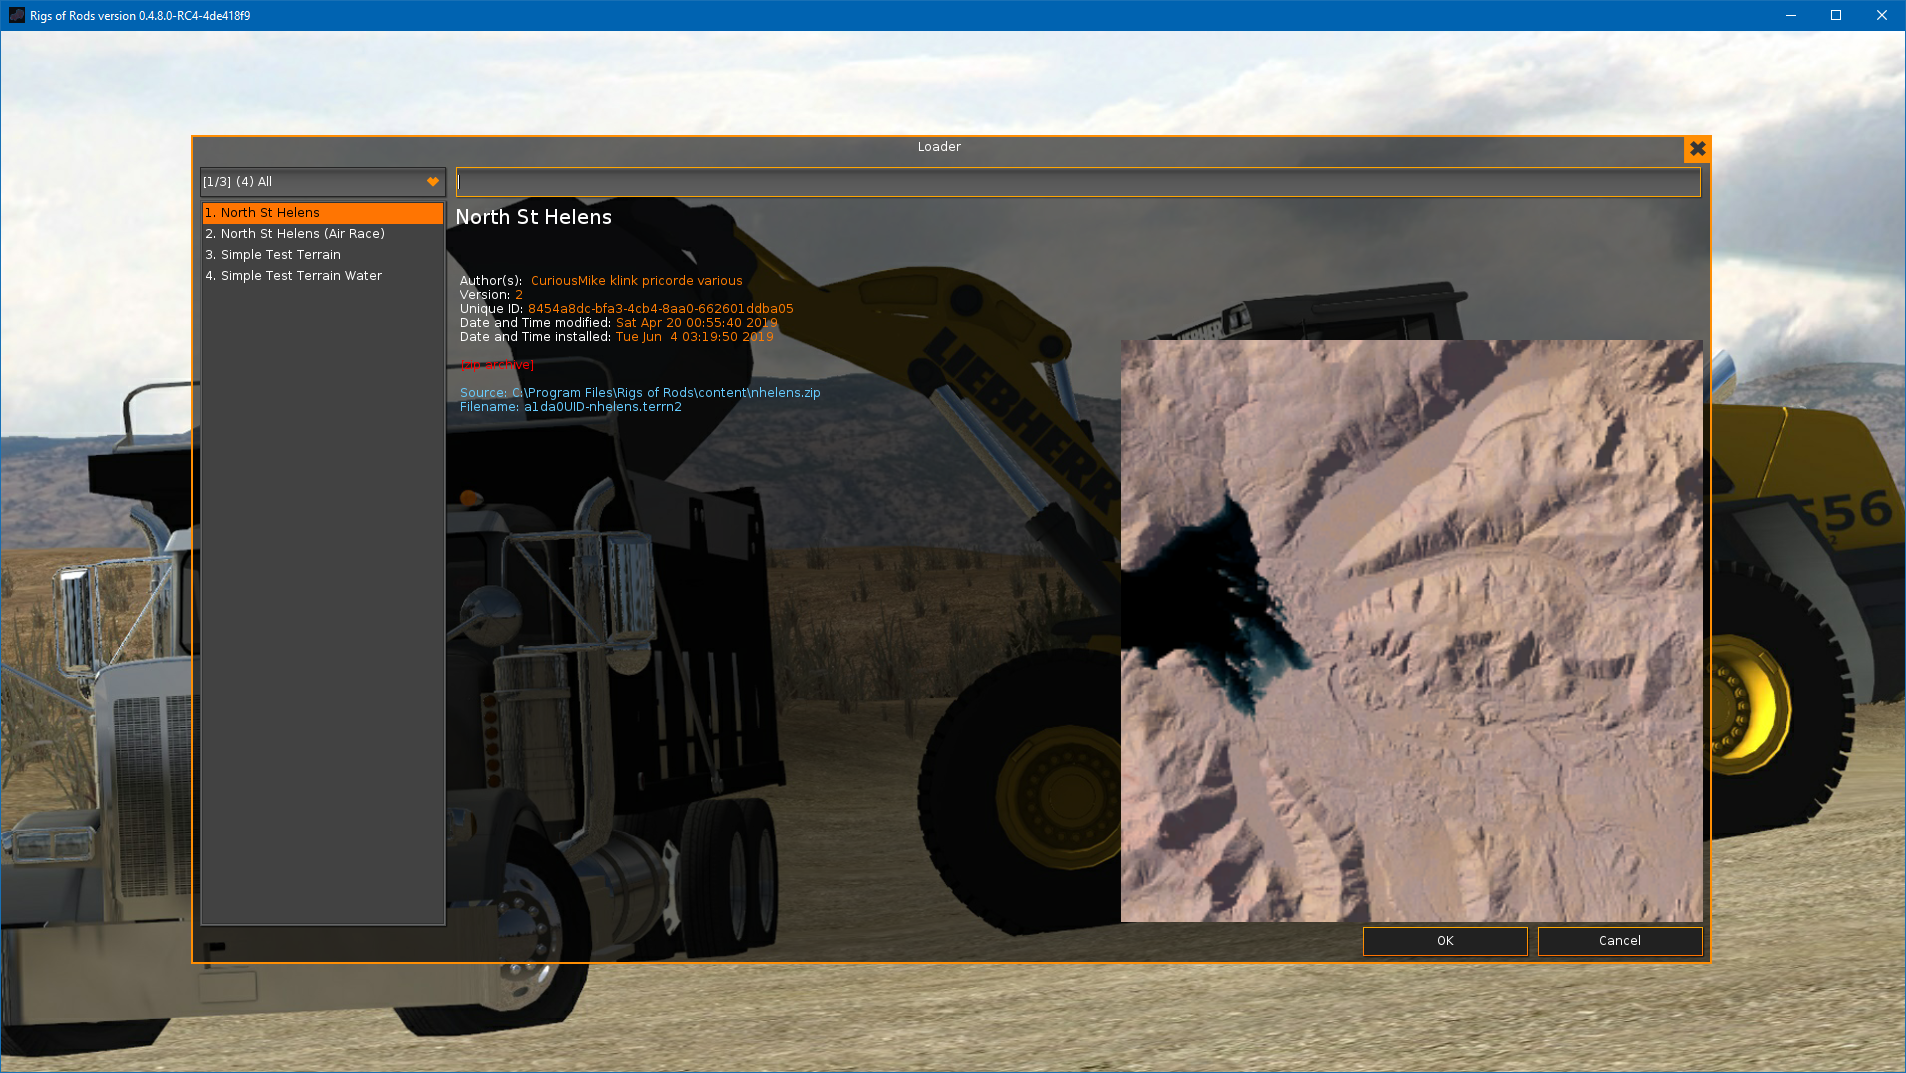
\includegraphics{images/bg-terrnselect.png}

For the sake of this tutorial, select \emph{North St Helens}.

Once the terrain loads, you will spawn as a country person known
lovingly as RoRBot. You control him with the arrow keys while using
\texttt{SHIFT} to run and \texttt{SPACE} to jump (good for getting over
bumps, or if you get stuck).

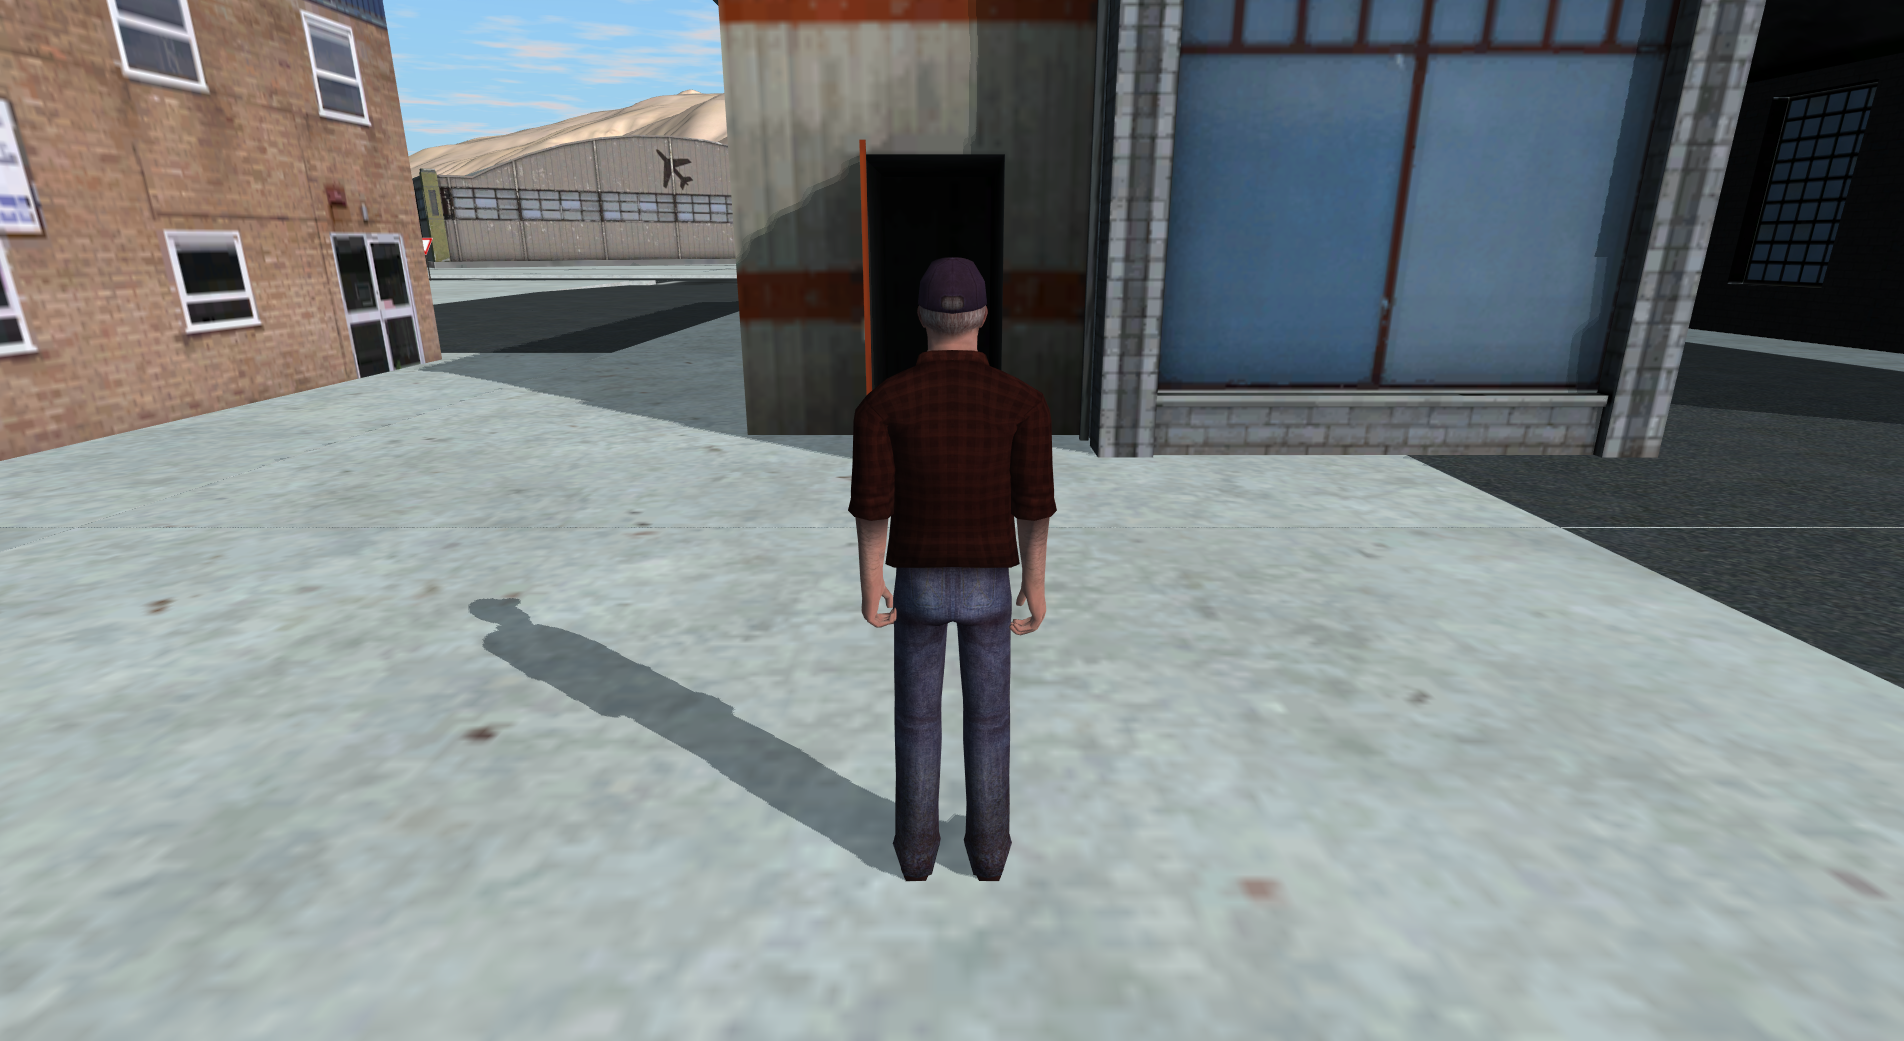
\includegraphics{images/bg-rorbot.png}

You spawn in front of a building known as the \emph{Rig-a-Deal}. This is
where you will spawn new trucks. Walk into the ``Office'' to bring up
the selection menu. You can also spawn a vehicle anywhere at any time by
pressing \texttt{CTRL+G}.

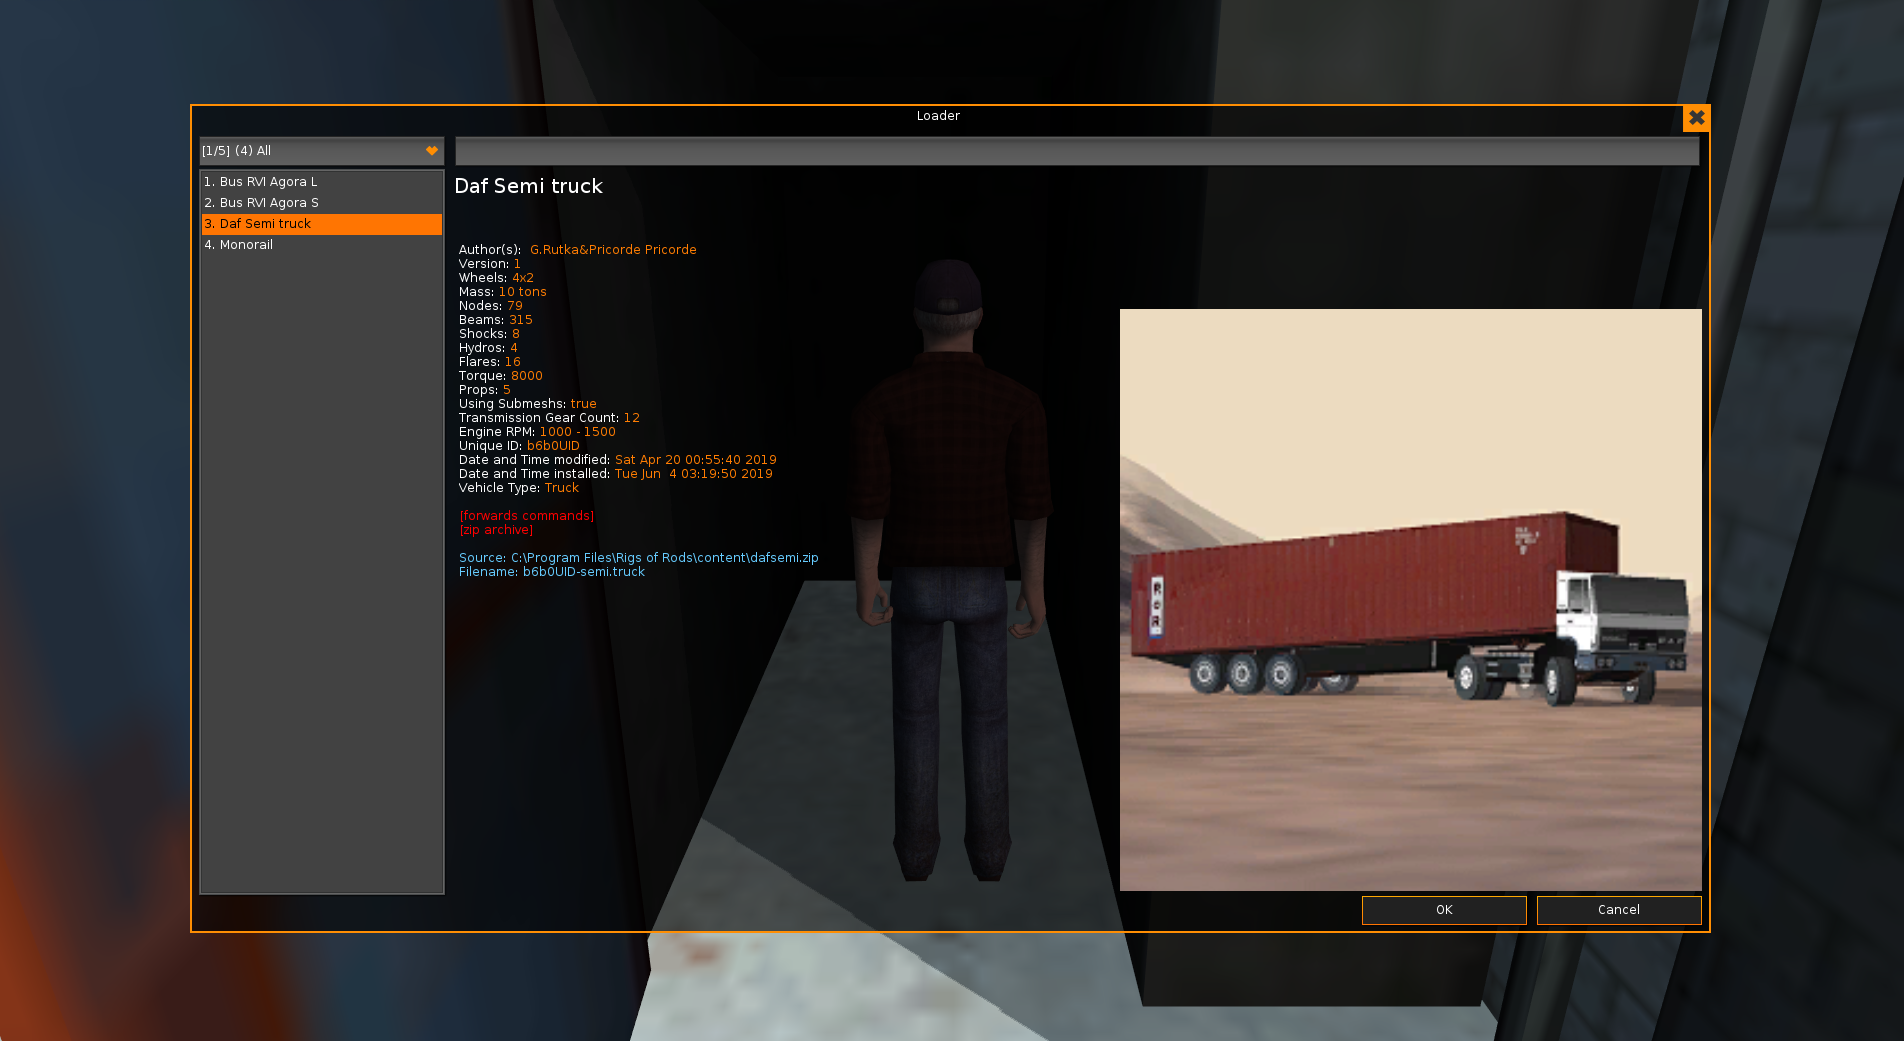
\includegraphics{images/bg-vehselect.png}

Use the mouse or arrow keys to move through the menus. Select the
\emph{DAF Semi truck}. The truck spawns inside the Rig-a-Deal with you
inside it. If you happen to spawn the truck with RoRBot outside of the
vehicle, simply hit \texttt{ENTER}/\texttt{RETURN} to get in a vehicle.

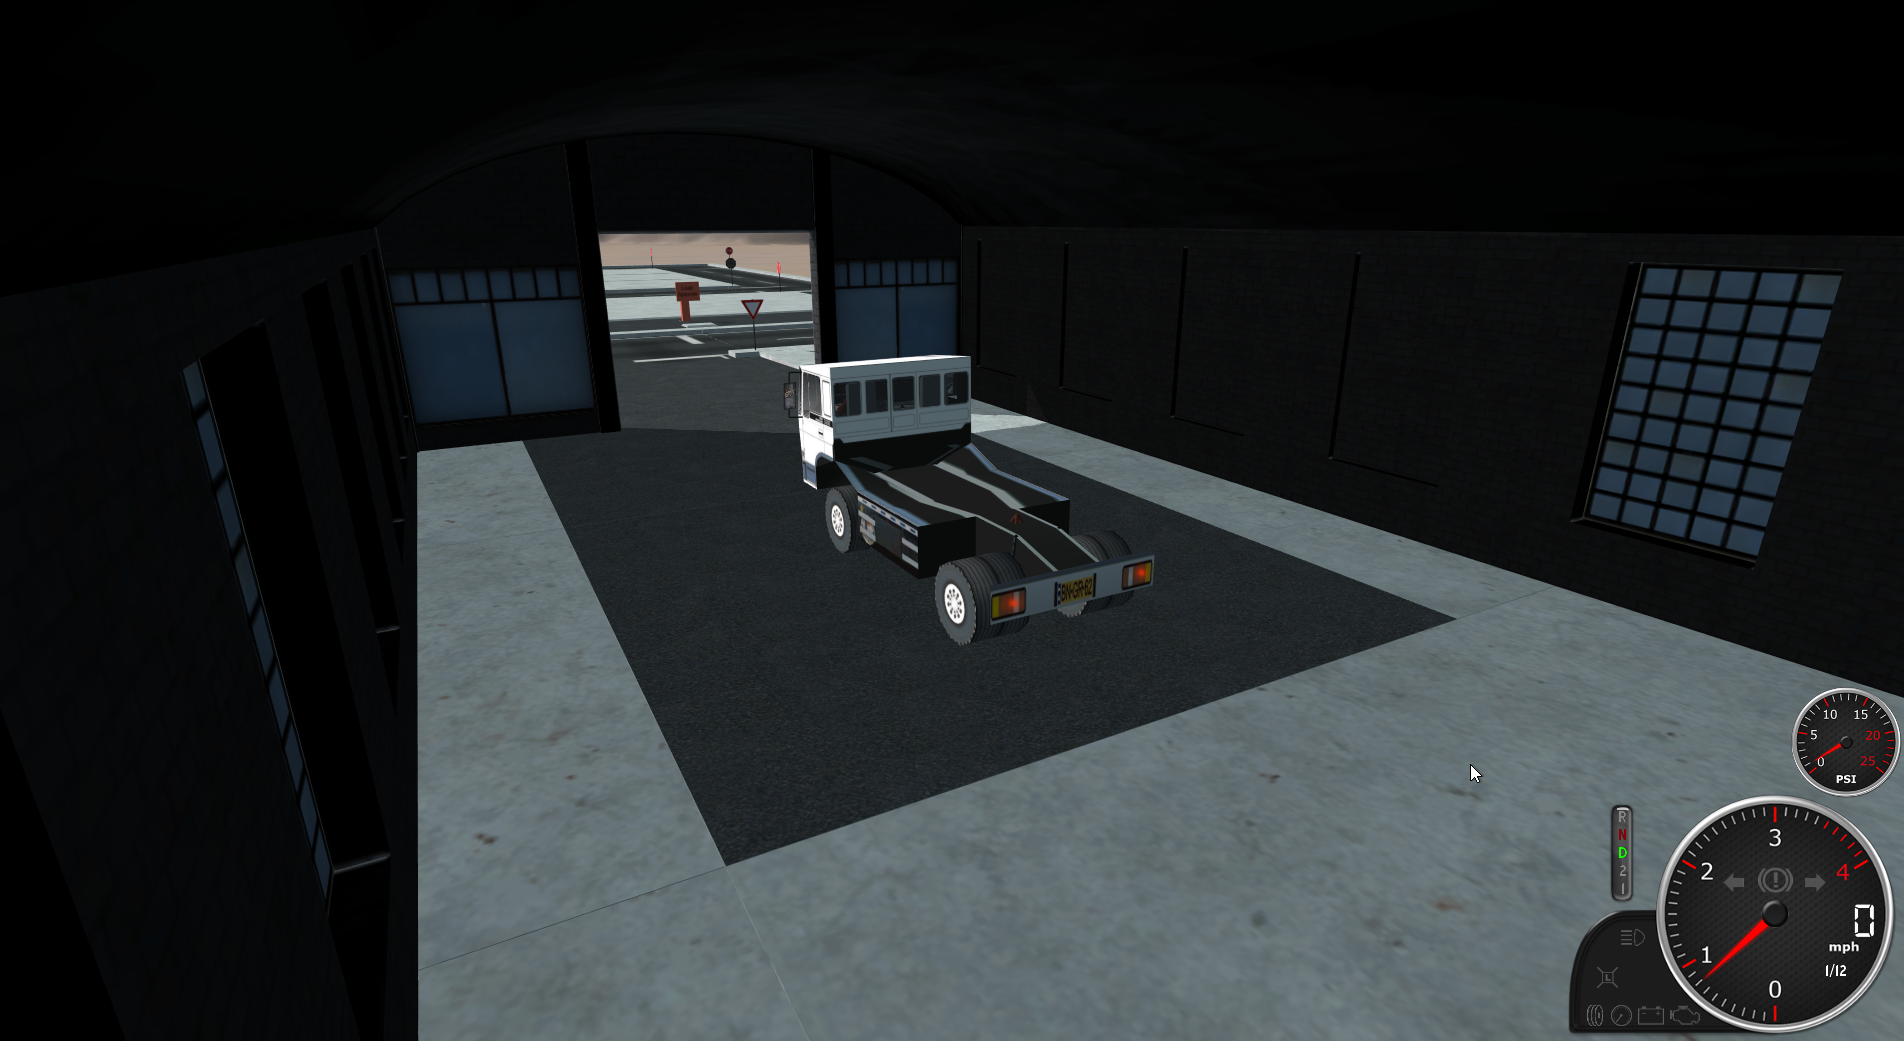
\includegraphics{images/bg-daf1.png}

\hypertarget{driving}{%
\section{Driving}\label{driving}}

The DAF semi isn't the most agile or best looking truck in the game, but
it serves us a purpose later. The camera inside the Rig-a-Deal is fixed,
so you will be unable to move it until you leave. Switch to the in-cab
camera by hitting \texttt{C}. Use the \texttt{UP} arrow key to
accelerate out of the \emph{Rig-a-Deal} (Rigs of Rods uses a simulated
clutch which begins to engages at a specific point. This why the semi
doesn't move until 1000 RPM). Use \texttt{DOWN} to brake, and
\texttt{LEFT}/\texttt{RIGHT} arrows to steer. Use
\texttt{PGUP}/\texttt{PGDOWN} to select your transmission
direction/speed.

Start by exploring Coldwater, the town you begin in. It isn't very big
but provides some decent moving room. If you get stuck, or wreck, hit
\texttt{I} to reset back to the \emph{Rig-a-Deal}, or \texttt{BACKSPACE}
to reset the truck in its current position.

If you hold \texttt{BACKSPACE} for one second, you will enable the
``advanced repair mode'' which lets you move the vehicle to any position
by using the \texttt{WASD} keys to move and the arrow keys to rotate.
Press \texttt{BACKSPACE} again to exit.

You can switch transmission modes by hitting \texttt{Q}. There are 5
transmission modes available: * Automatic shift * The gear change is
fully automatic, the player only has to set the gear by pressing
\texttt{PGUP}/\texttt{PGDOWN}. * Manual shift: Auto clutch * The gear is
changed on user request. No clutch should be pressed to change gear,
vehicle takes care of that. Just use \texttt{A} and \texttt{Z} to shift.
* Fully manual: sequential shift * The user must press clutch and select
whether it is needed to switch up or down. Depress the clutch by hitting
\texttt{LEFT\ SHIFT}, then press \texttt{A} to upshift or \texttt{Z} to
downshift. * Fully manual: stick shift * This mode is useful if you have
a game controller with an H-shifter (like Logitech G27). In this mode
the player can set gears 1-6, N, and R directly by the stick. * Fully
manual: stick shift with ranges * This mode is mostly used in vehicles
having more gears than 6. In this case you can select from 3 ranges: low
(gear 1-6), medium (gear 7-12), high (gear 13-18) by pressing the
appropriate button. Like if you want to select the 8th gear, you have to
select gear N first, press the midrange button, then select the 2nd gear
on the h-stick. Remember, range selection can be made only if the gear
is in N.

If you stall, there are 2 keys to be remembered: \texttt{X} enables or
disables the electricity in the vehicle, and \texttt{S} activates the
starter. Press \texttt{X} and you'll see a yellow battery icon lit on
the UI. Hold \texttt{S} until the engine is started. Resetting the
vehicle with \texttt{BACKSPACE} or \texttt{I} will instantly start the
engine.

Remember how to change the camera? Hit \texttt{C} twice. You're now in
third-person view and can move the camera around. Use the number pad
(specifically \texttt{2}, \texttt{4}, \texttt{6}, and \texttt{8}) to
move the camera. Pressing \texttt{5} resets the camera. \texttt{9} and
\texttt{3} zoom in/out respectively and \texttt{1} gives you a front
view of your truck.

You can also move the camera by holding right-click and dragging with
your mouse.

Now, make your way back to the \emph{Rig-a-Deal}.

\hypertarget{trailer-loads}{%
\section{Trailer Loads}\label{trailer-loads}}
You should see a large, grey, open-platform with an orange console. Park
the truck (use \texttt{P} to set the parking brake) and hit
\texttt{ENTER}/\texttt{RETURN} to get out. Note that the same camera
commands work with RoRBot. Step in front of the orange console to open
the load selector.

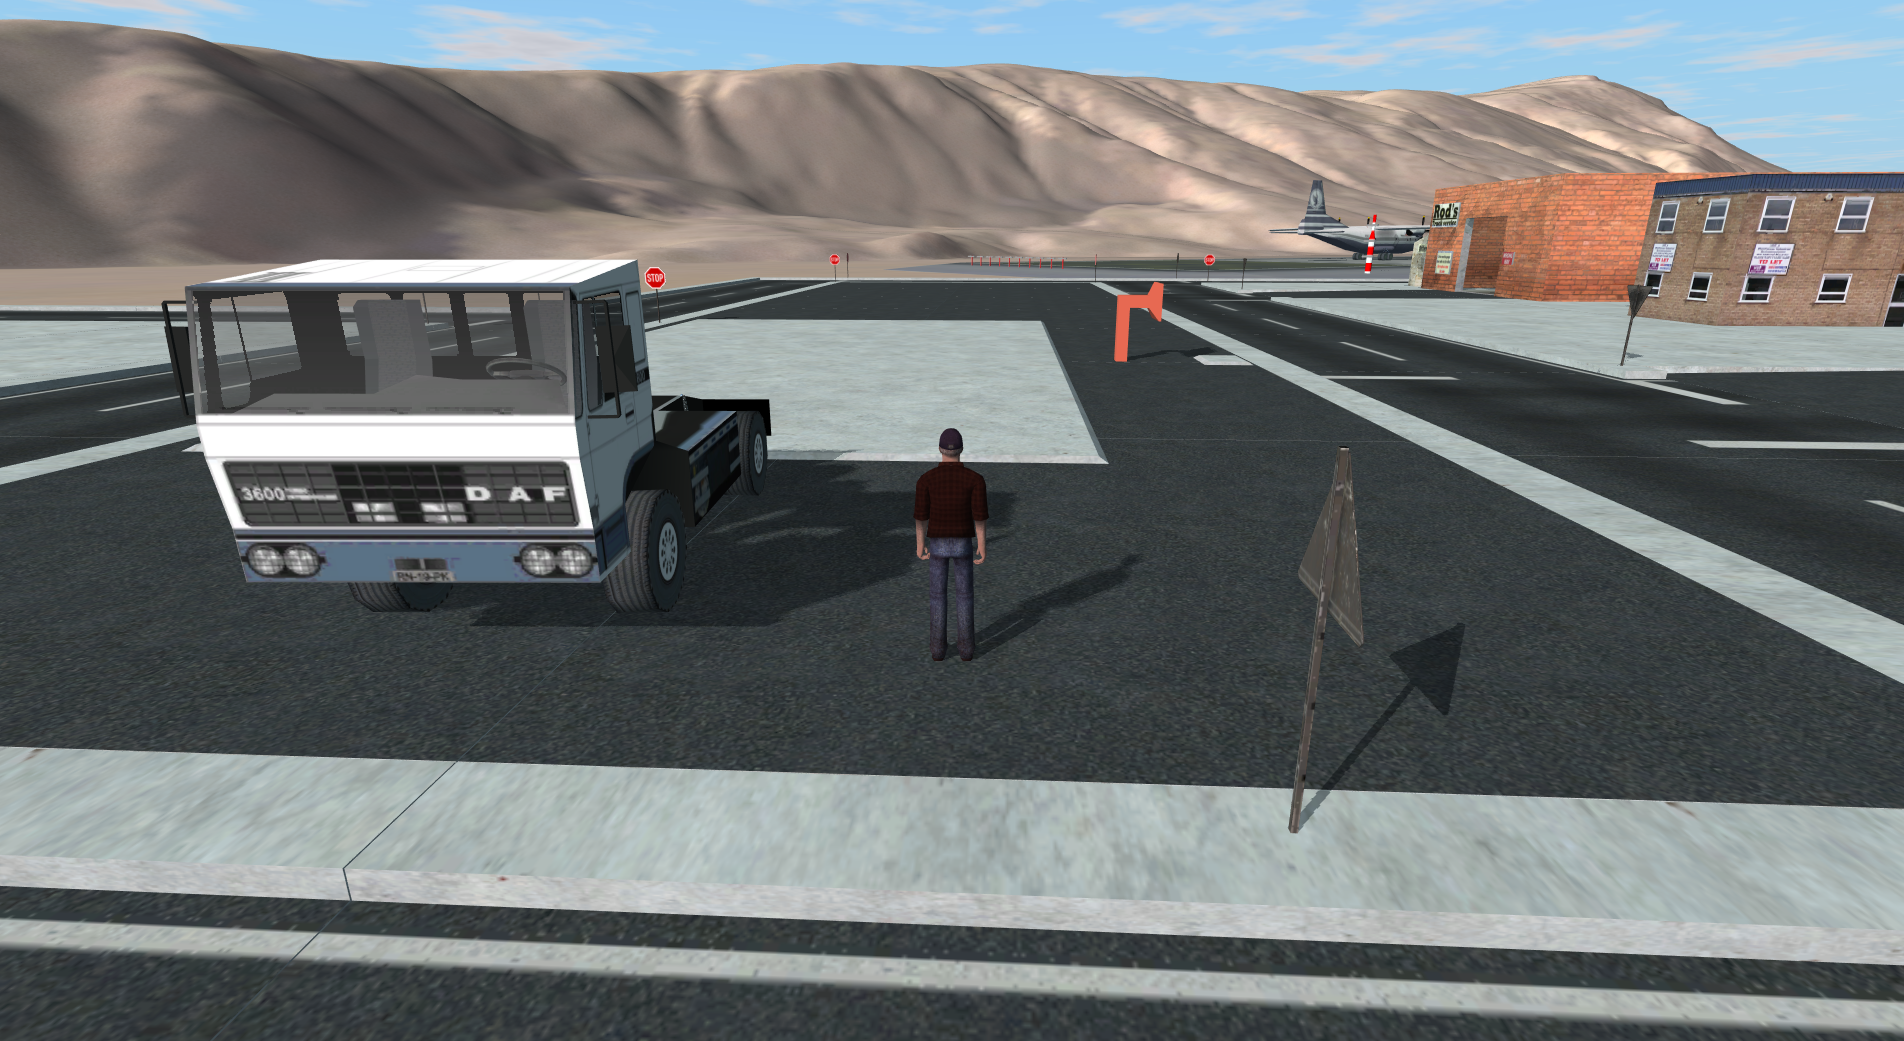
\includegraphics{images/bg-daf2.png}

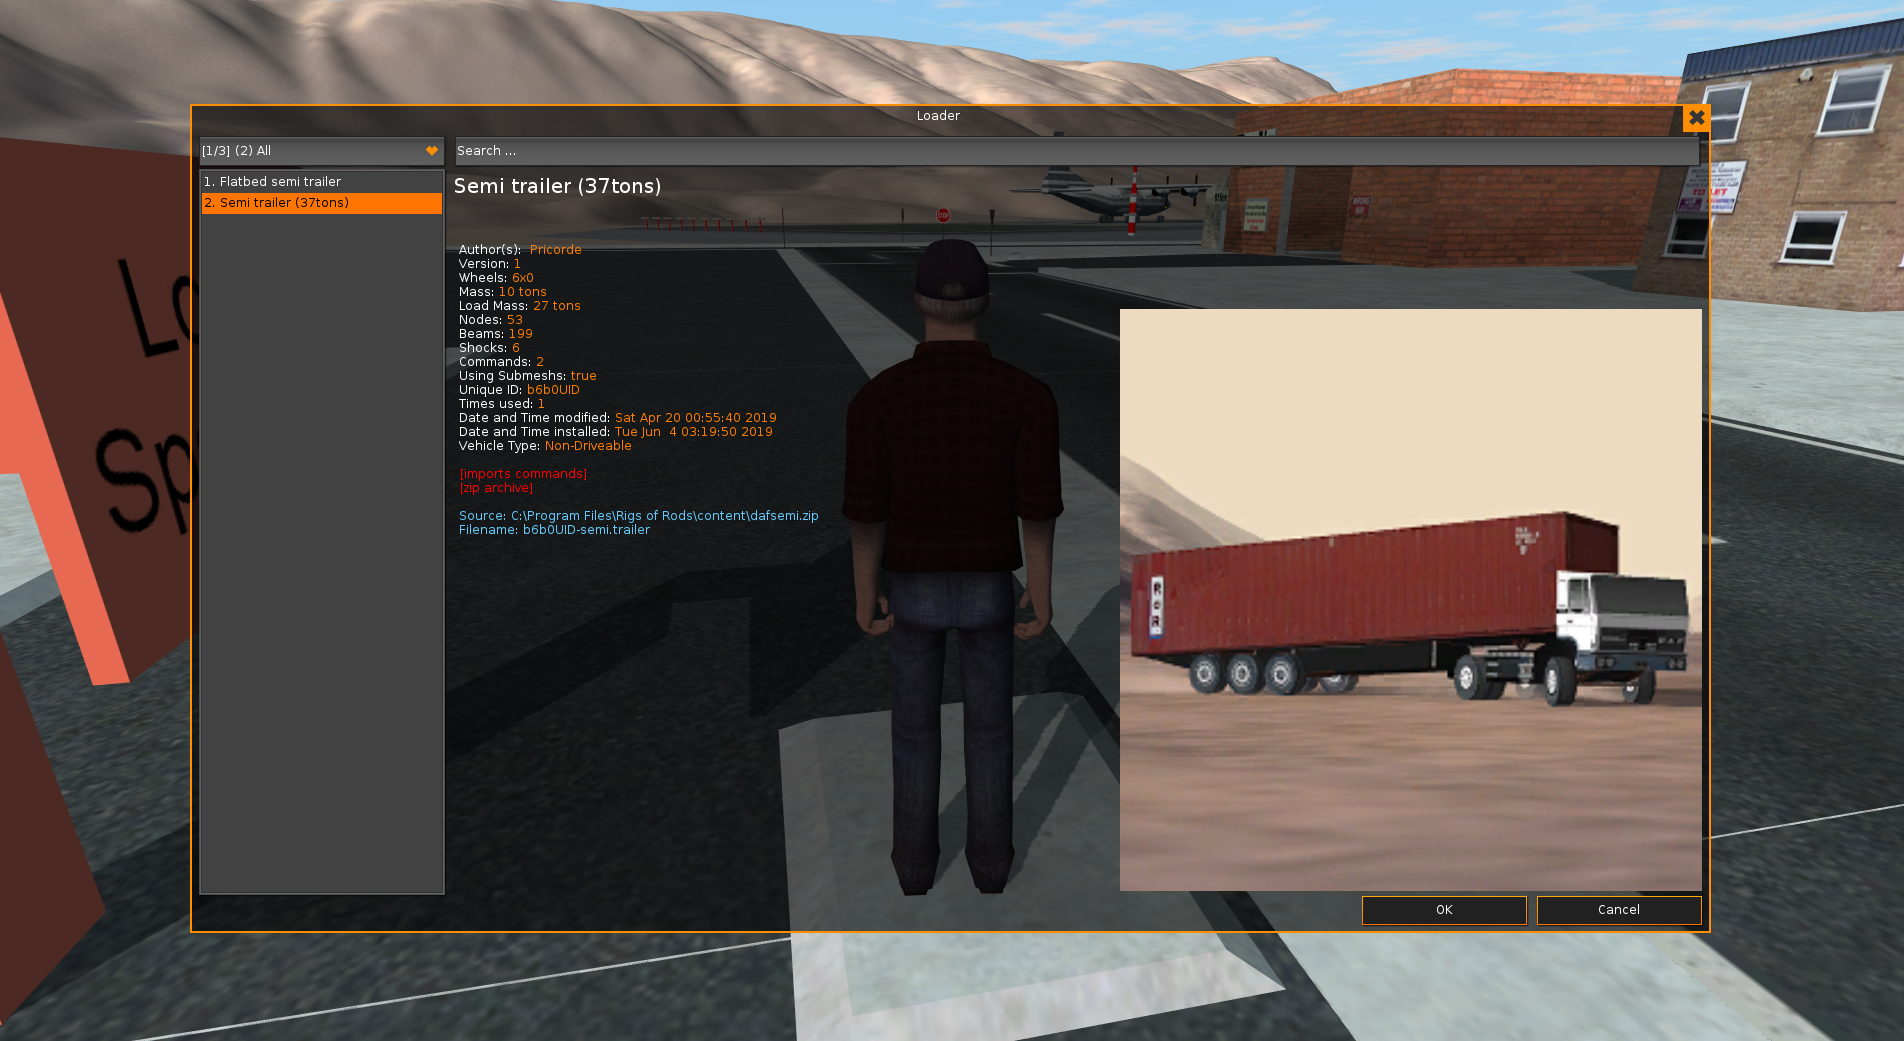
\includegraphics{images/bg-loadselect.png}

Select the \emph{Semi trailer (37 tons)}.

Get back in the semi and drive in front of the load. Use the camera in
third-person view to help you if you need. Back into the trailer. When
you get close, use \texttt{F1}/\texttt{F2} to lower and raise the
trailer legs respectively.

The hook points must be within 10cm to hook, so it may take some
practice to get close. When you think you're close, hit \texttt{L}. If
you're close enough, the semi will latch to the trailer. Raise the legs
by holding \texttt{F1}.


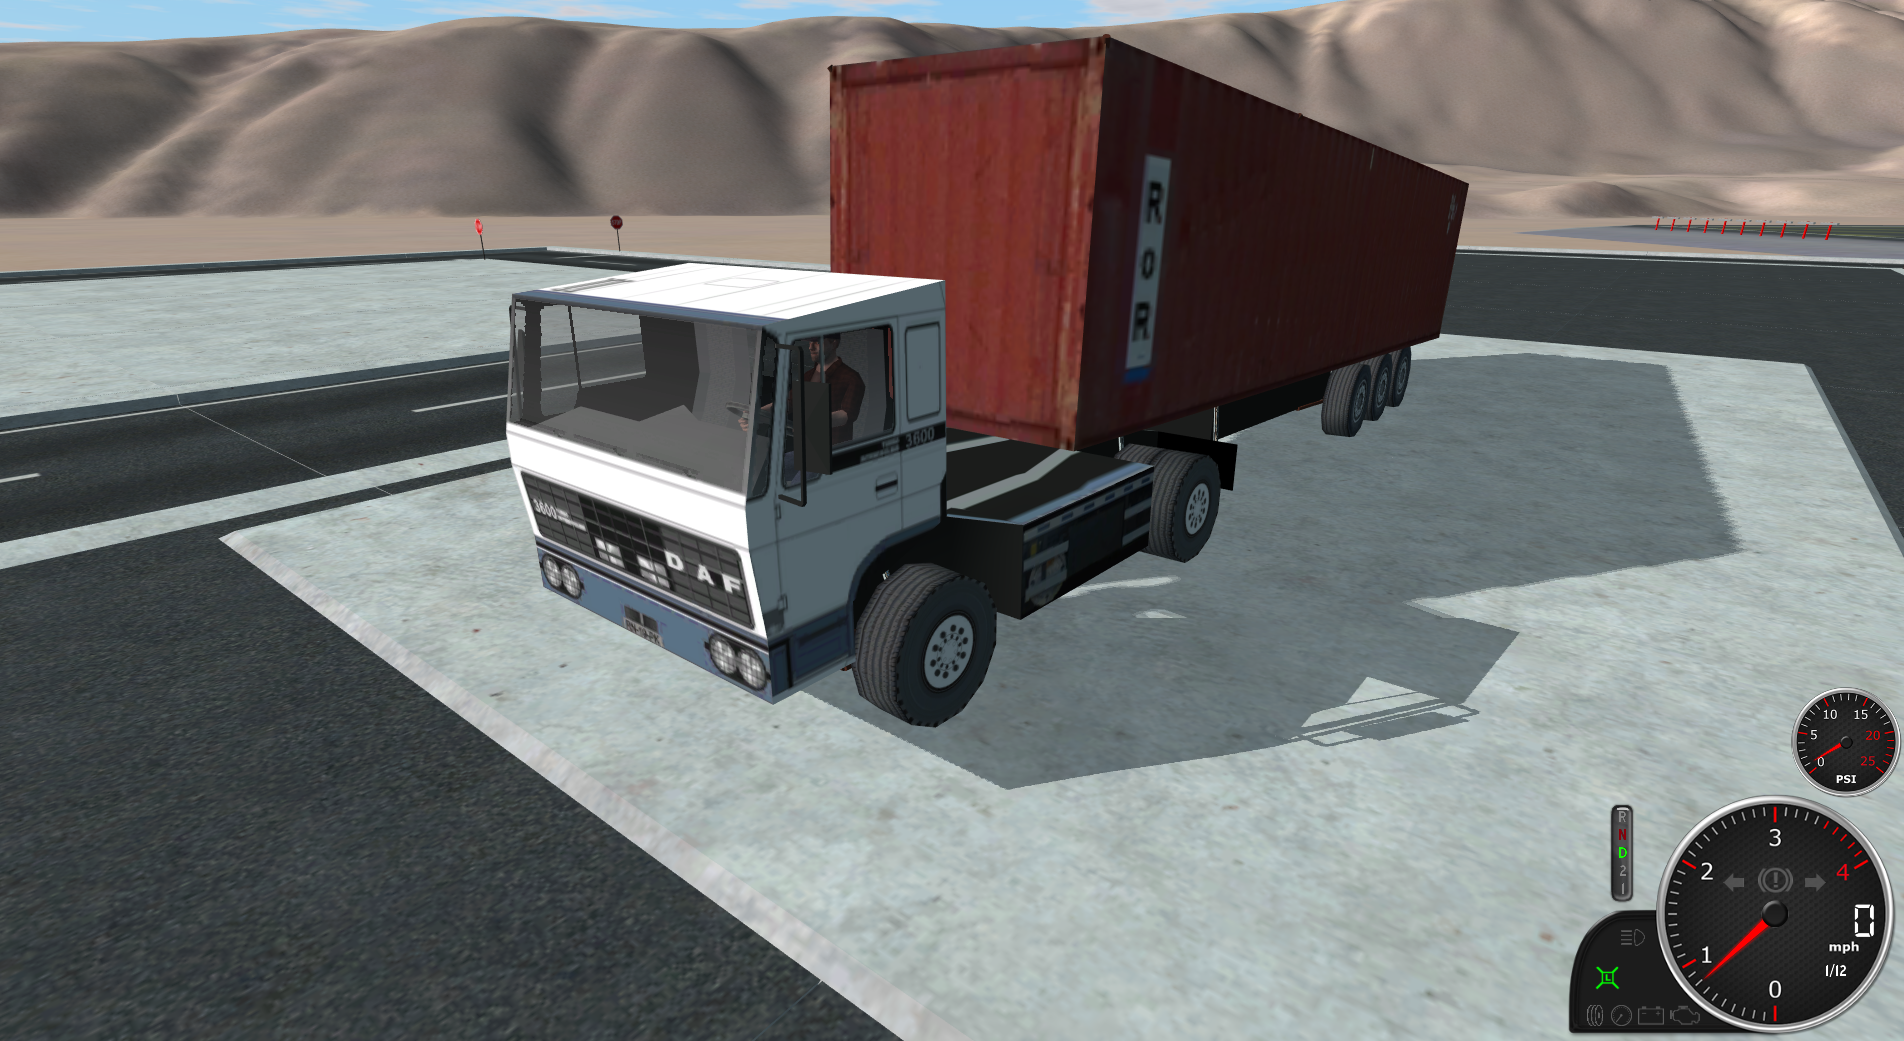
\includegraphics{images/bg-daf3.png}

You can now drive around with the trailer. You will notice that the
trailer has a large effect on how the semi pulls and handles! This
process is the same for most trailers. In some cases you can secure
loads to trucks using \texttt{O}.

NOTE: on some computers trailers may increase lag or decrease FPS(frames
per second) dramatically!

\hypertarget{flying}{%
\section{Flying}\label{flying}}

Now that we've become comfortable with driving. Let's try to fly. Move
your mouse to the to top of the screen to bring up the menubar, click
\texttt{Vehicles} then \texttt{Antonov\ 12} to instantly enter the plane
which is sitting on the runway.


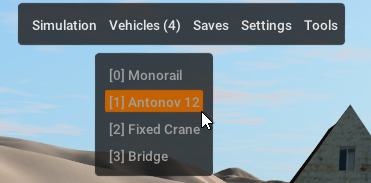
\includegraphics{images/bg-planeselect.png}


Apply the parking brake by pressing \texttt{P}. Turn on the flying
lights by pressing \texttt{M}. Start the engines by using your mouse to
click the \texttt{ON} buttons in the lower right hand corner (or by
pressing \texttt{CTRL+HOME}).

When the engines settle to the appropriate idle speed (somewhere near
750rpm), release the parking brake and throttle the engines to full by
holding \texttt{PGUP}. Pressing \texttt{CTRL+PGUP} will instantly set
the throttle to max.

If you have a short runway, be sure to use the flaps with \texttt{1} and
\texttt{2} (this is especially helpful in multiplayer). When you reach
75-80 knots, lift up by pressing the \texttt{DOWN} arrow. Steer with the
\texttt{LEFT}/\texttt{RIGHT} arrows and control the rudder with
\texttt{Z} and \texttt{X}. Raise the landing gear, in this plane, by
holding \texttt{F3}.

The An-12 does not stand high speeds (175+ knots) well, and you may find
that if you go too fast the wings will break apart!

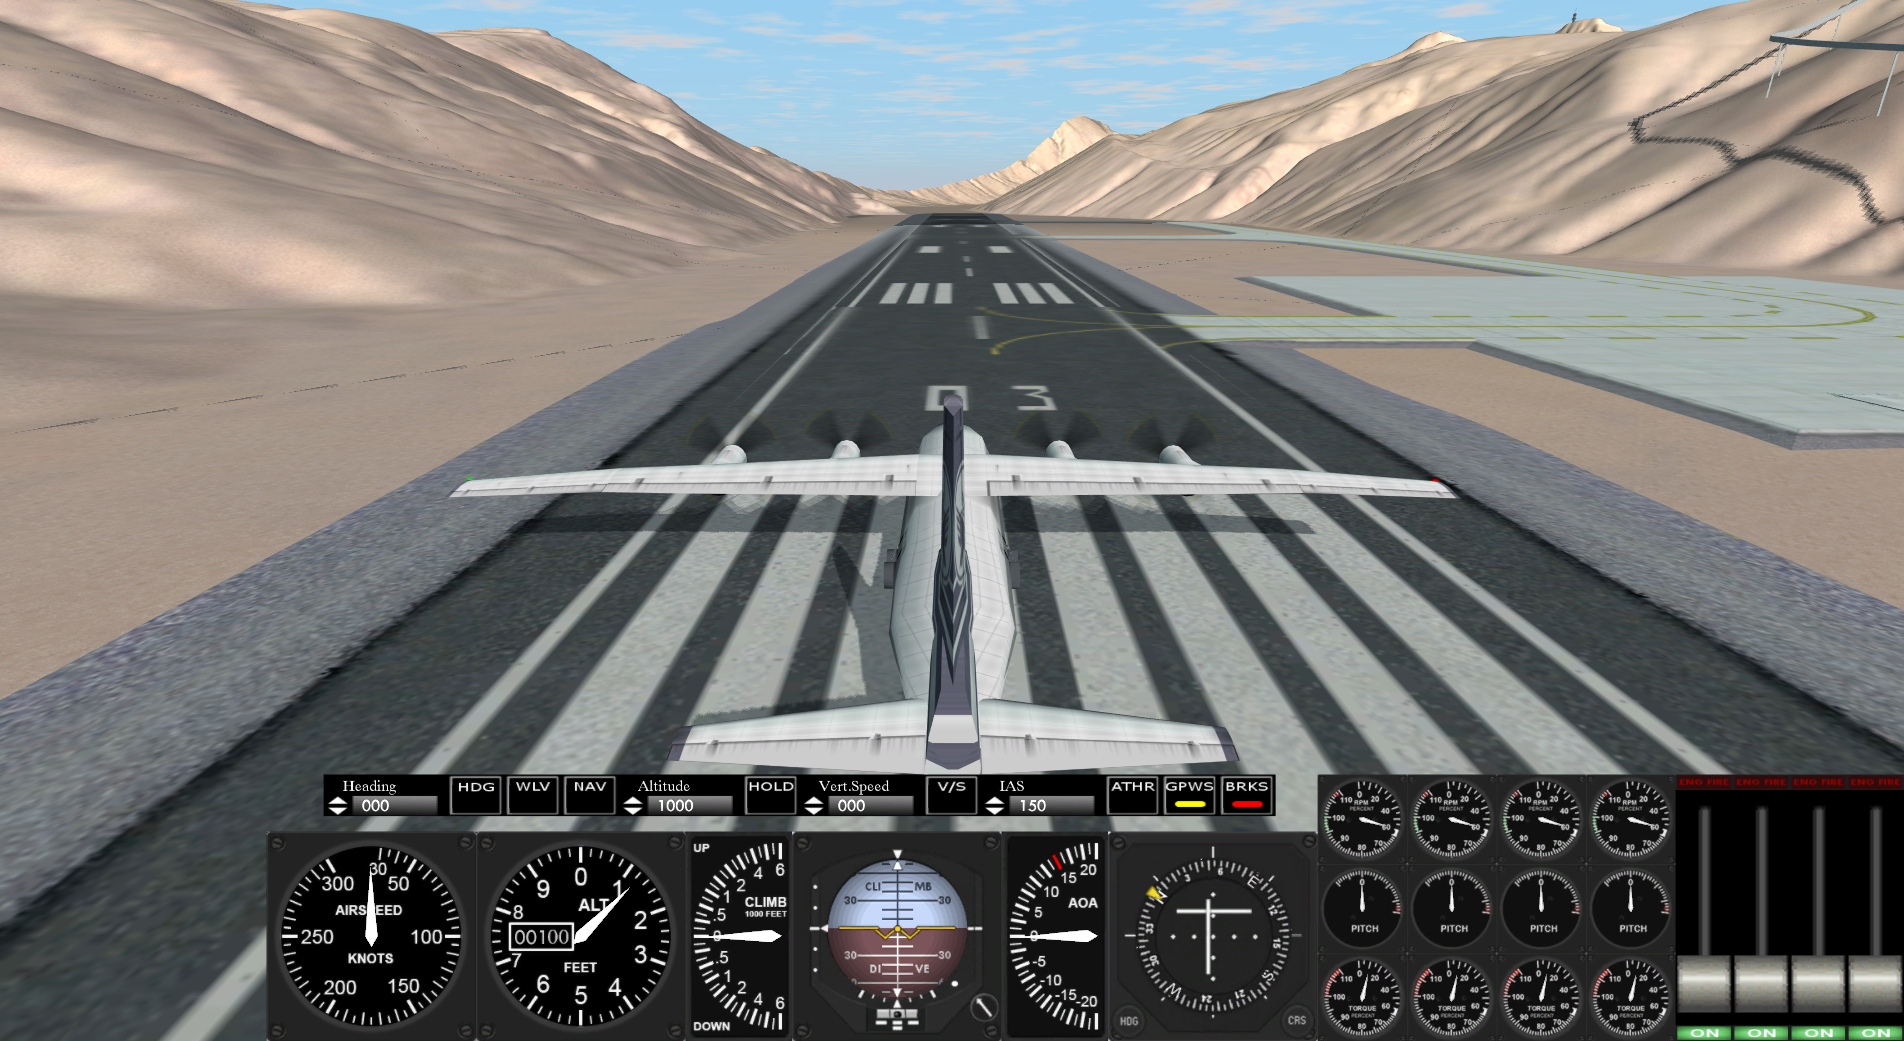
\includegraphics{images/bg-plane1.png}

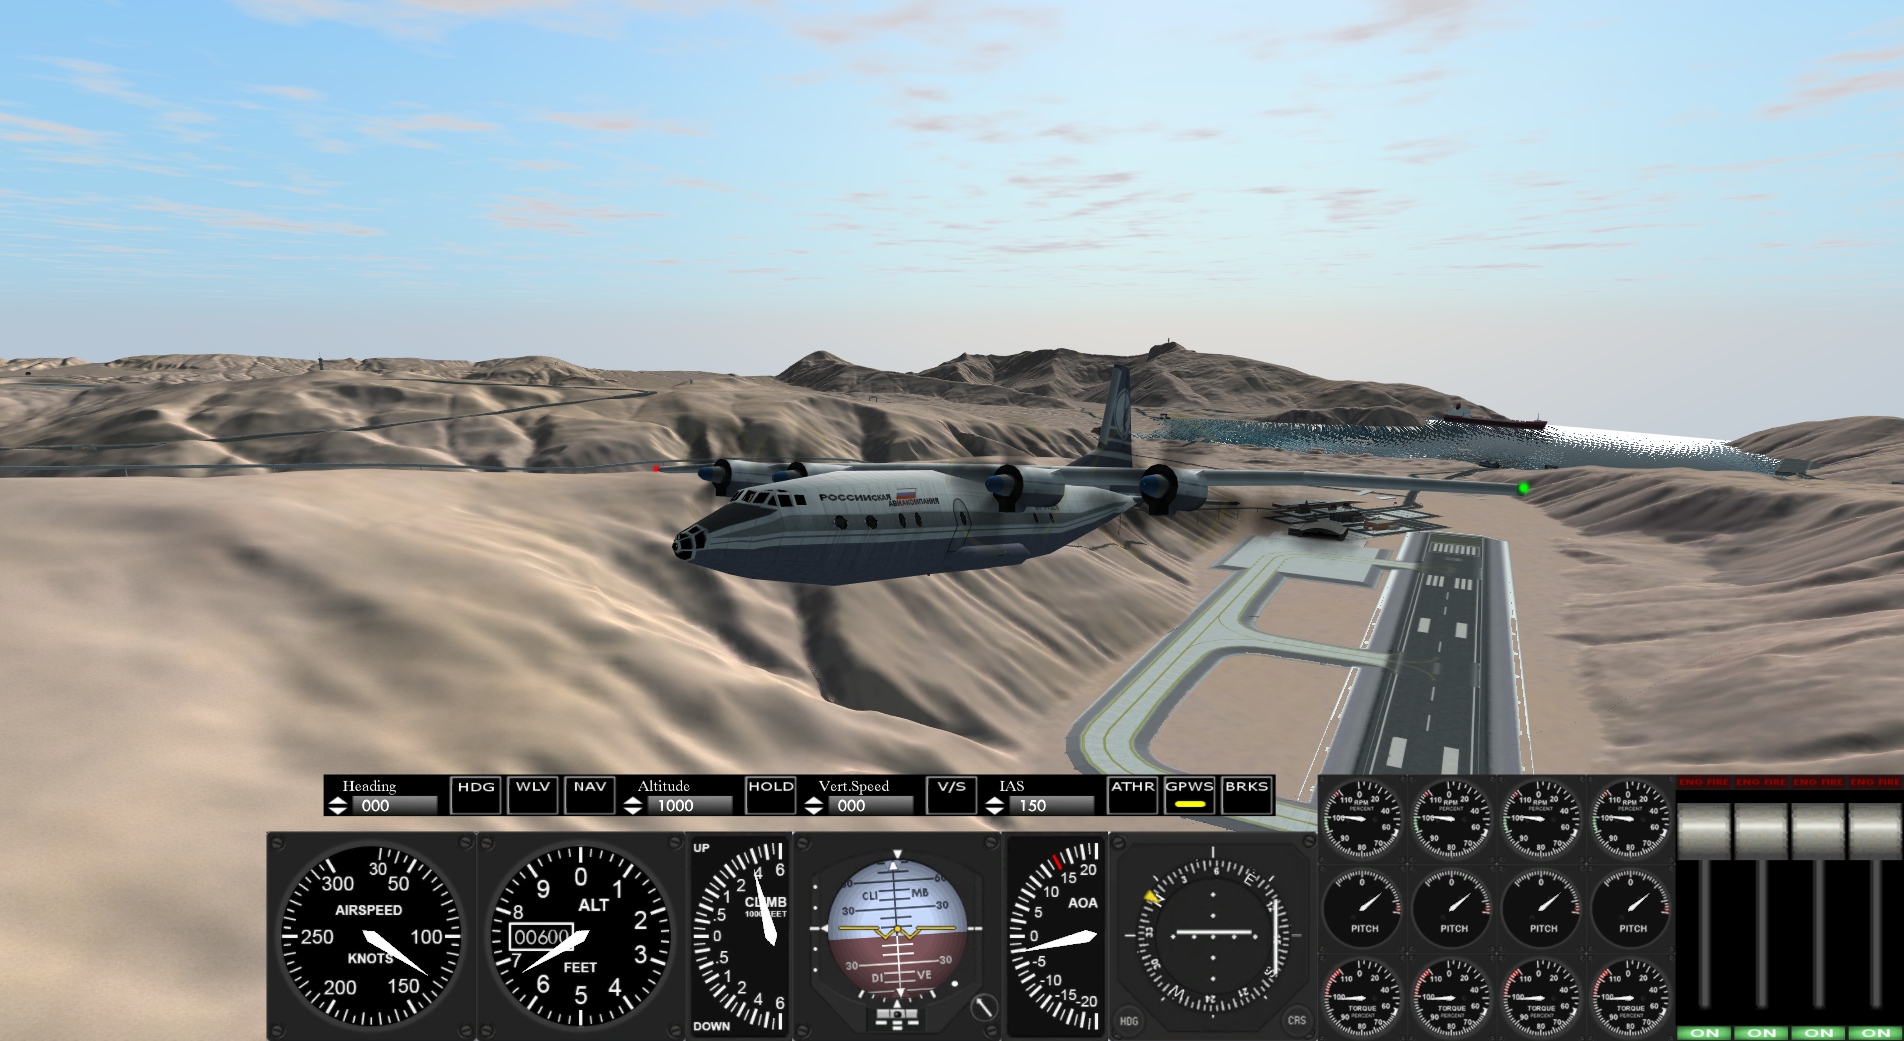
\includegraphics{images/bg-plane2.png}

When it comes to landing, make sure you have room to slow down and take
your time. Going straight into the runway is the easiest way to land
when you first start off. It may take a few passes to go head-on so
don't be afraid to abort a landing and throttle back up to regain
altitude. The entire process is easier if you shadows enabled, but is
possible without. When you land, hit \texttt{R} to reverse thrust and
throttle up to slow down in addition to using \texttt{B} to brake the
wheels.

This tutorial does not make use of the autopilot. For more information
regarding the use of autopilot, see
\href{/gameplay/aircraft-handling/}{Aircraft handling}.

\hypertarget{boating}{%
\section{Boating}\label{boating}}

We must explore beyond Coldwater to get to the marina. Take the main
road out of Coldwater, heading southwest toward the Elk Hotel. Take the
second left after you leave town. You should see the water soon. When
you arrive at the marina, you should see marina-style boat docks and a
ramp along with a building.

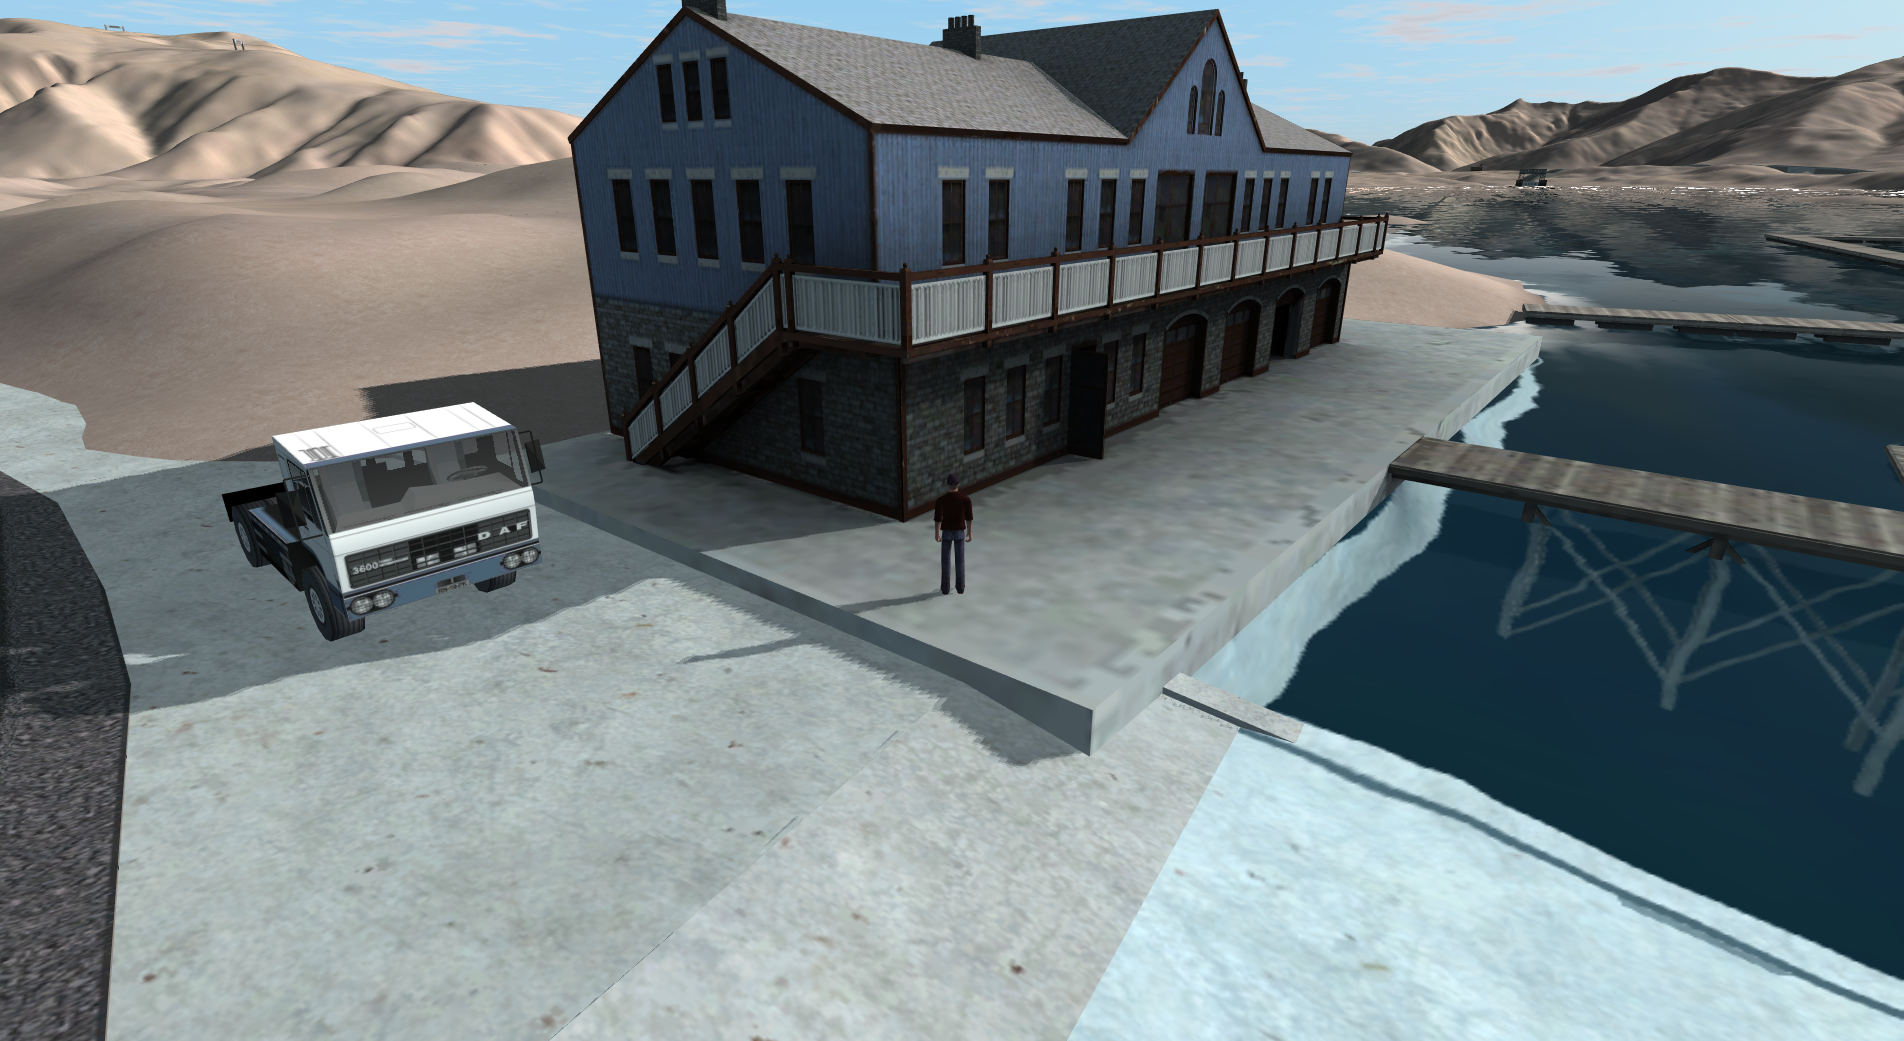
\includegraphics{images/bg-boat1.png}

Walk around to the front of the building and enter the open door. Choose
the Wahoo boat.

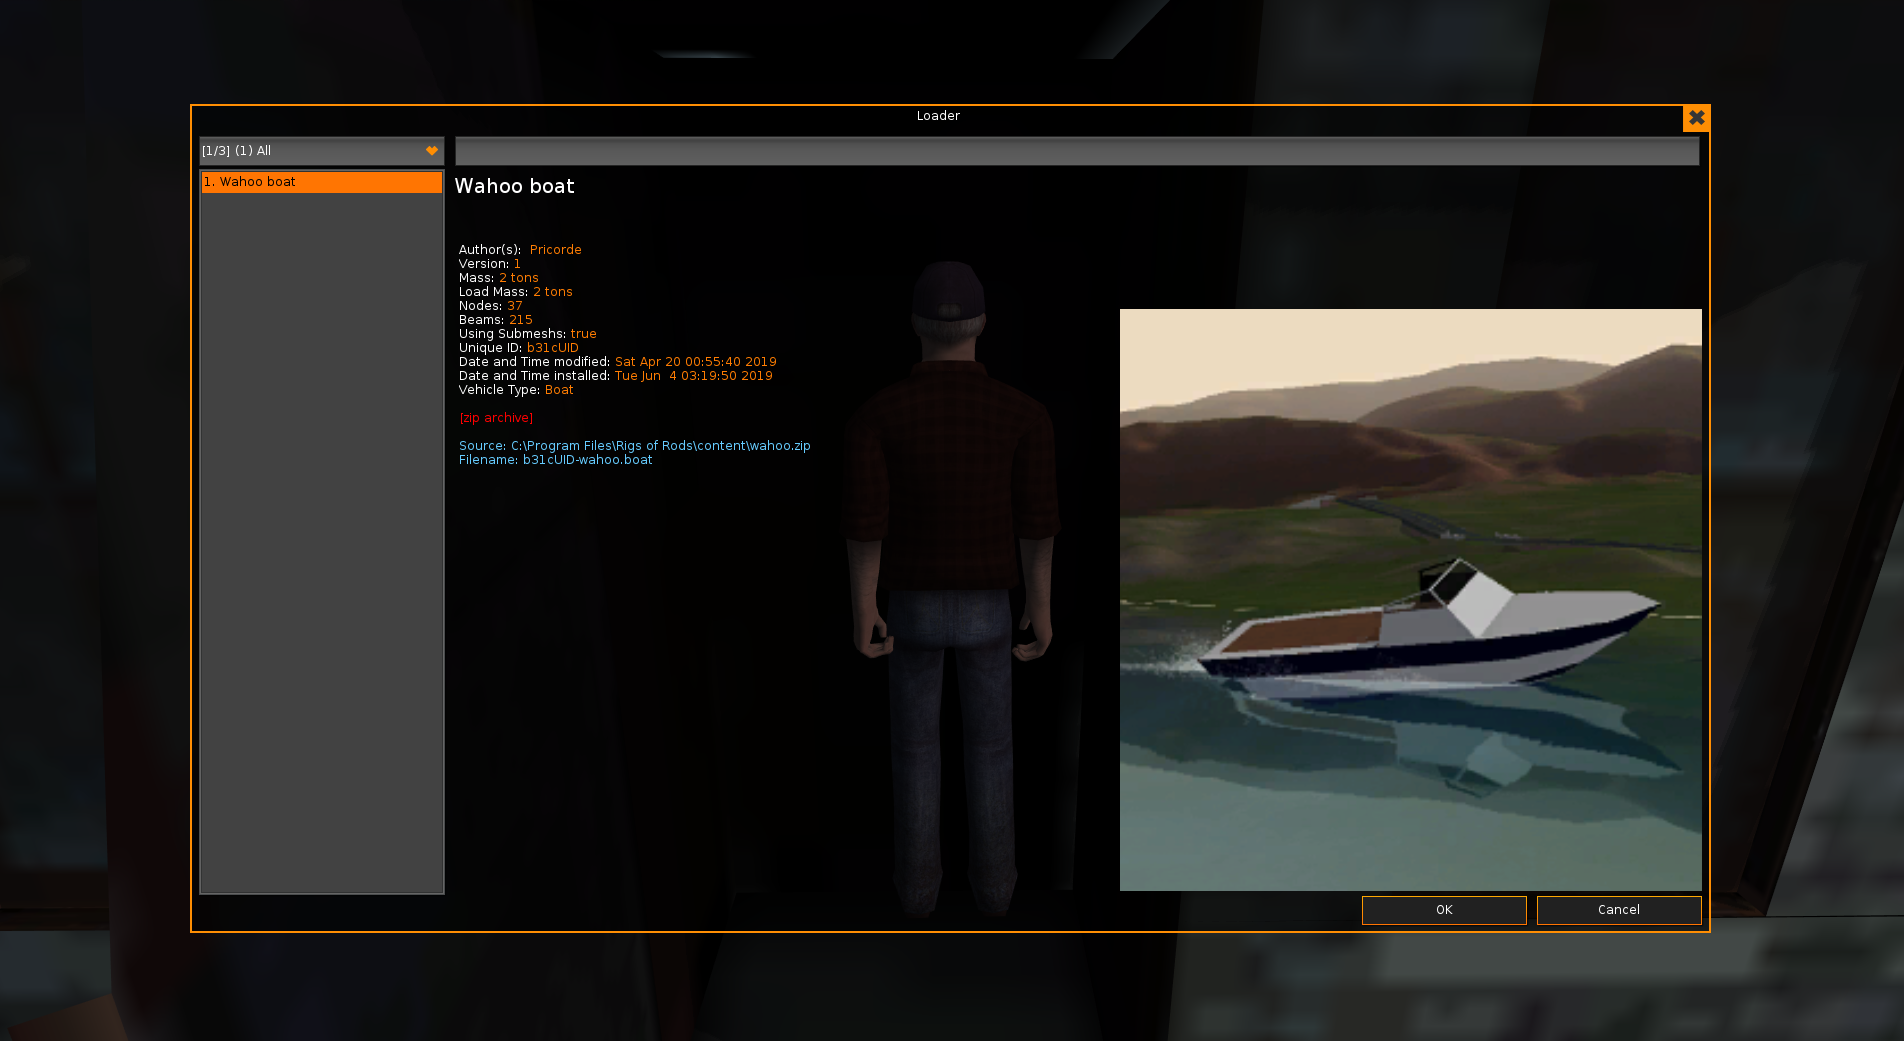
\includegraphics{images/bg-boatselect.png}

Use \texttt{UP}/\texttt{DOWN} to throttle and
\texttt{LEFT}/\texttt{RIGHT} to steer. Use \texttt{PGUP} to center the
throttle (to neutral) and \texttt{PGDOWN} to center the rudder. It may
take you a while to get your sea legs. If you have waves enabled, see
how far out you can go before you flip over waves!

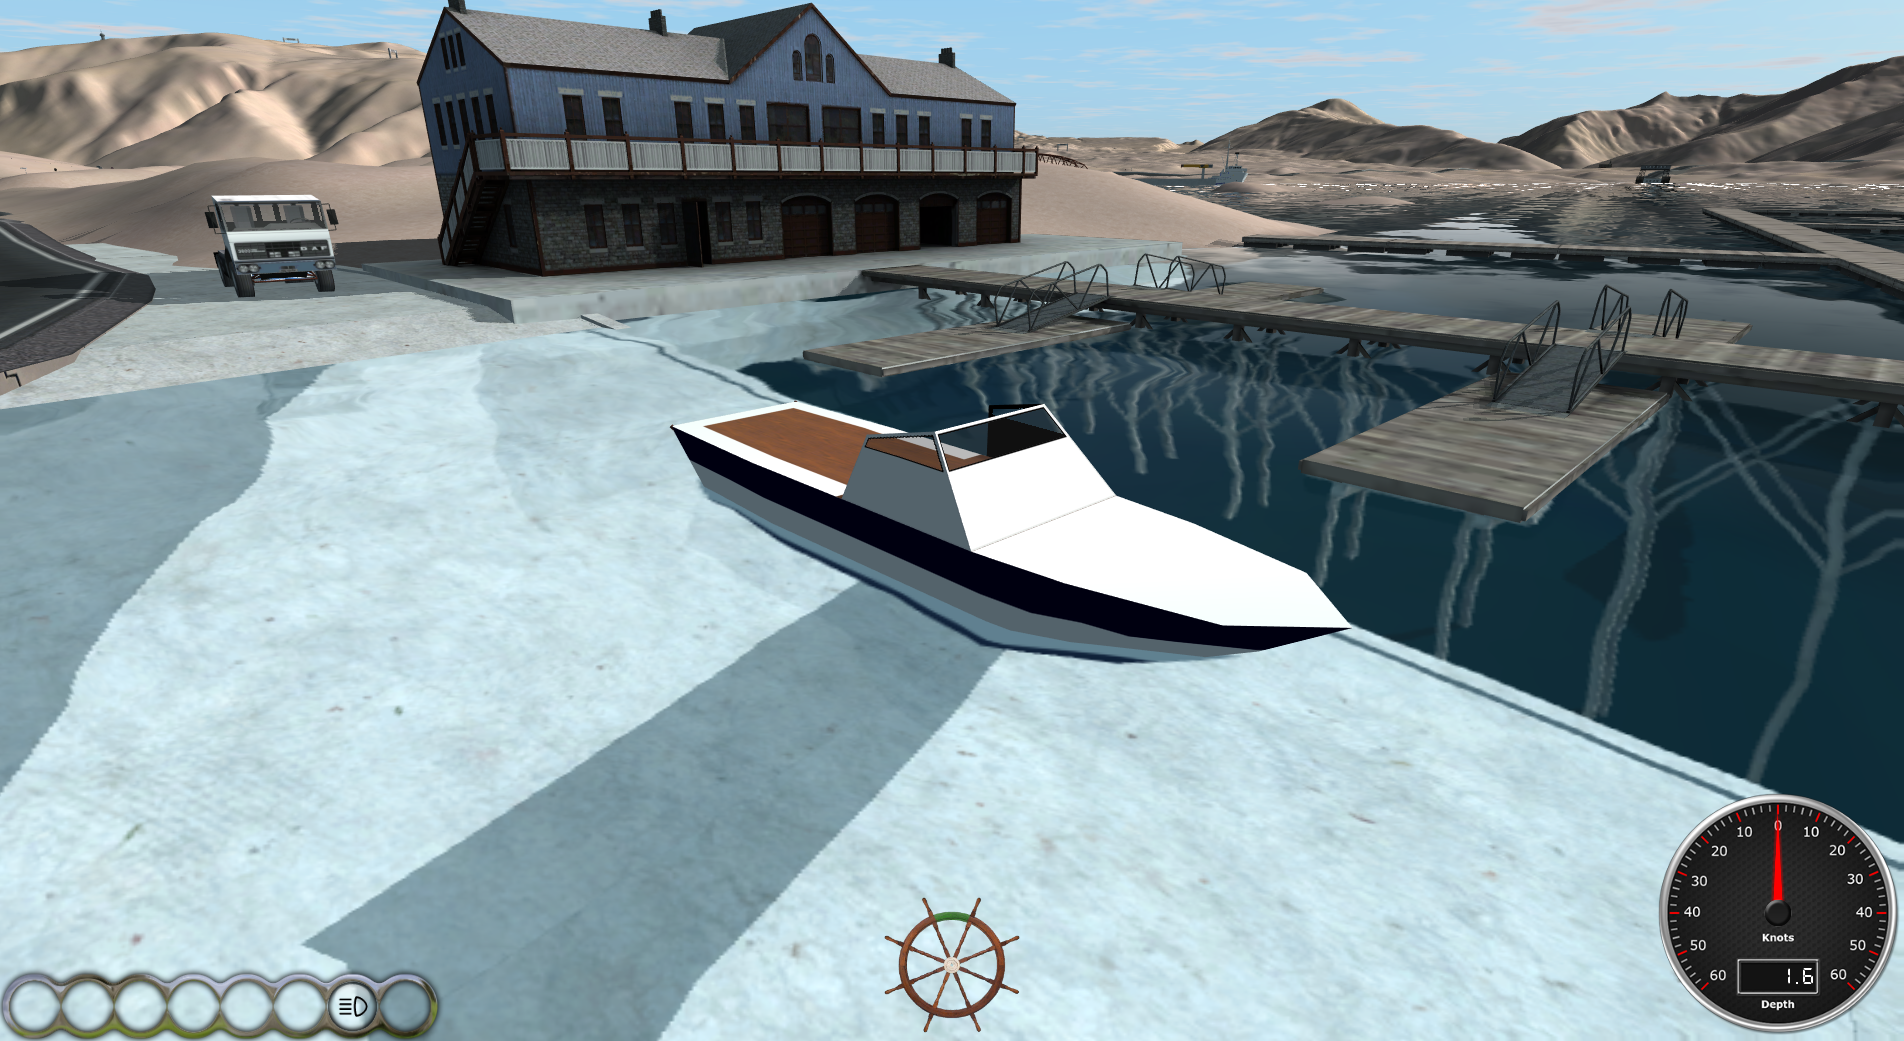
\includegraphics{images/bg-boat2.png}

\hypertarget{conclusion}{%
\section{Conclusion}\label{conclusion}}

Now that you have a basic grasp of the basic vehicles in RoR, it is now
up to you to create your own scenarios. If you feel bored, try the vast
selection of mods available on the
\href{https://forum.rigsofrods.org/resources/}{Repository}.

\hypertarget{multiplayer}{%
\section{Multiplayer}\label{multiplayer}}

If you feel like sharing the experience, you can play on one of the many
public multiplayer servers. To get started, click the
\texttt{Multi\ player} button on the main menu.

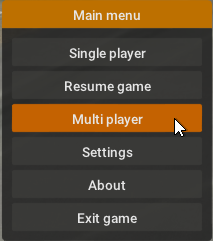
\includegraphics{images/bg-mp1.png}

Set your username by clicking on \texttt{Settings} and changing it in
the \texttt{Player\ nickname} textbox.

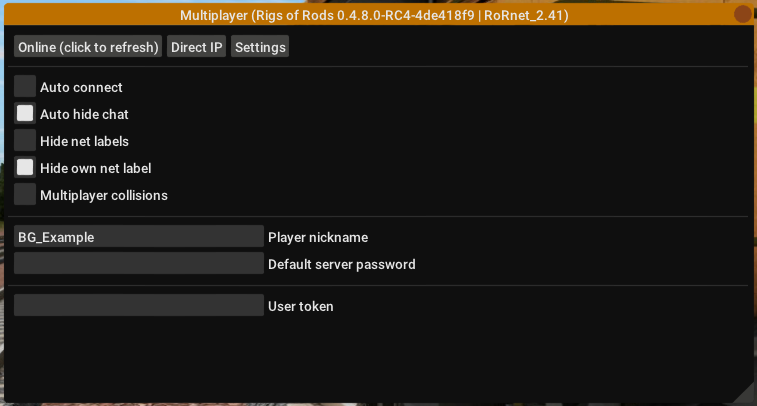
\includegraphics{images/bg-mp2.png}

You may have to restart the game for the changes to take effect.

Now just select the server you want to play on, then click
\texttt{Join}.

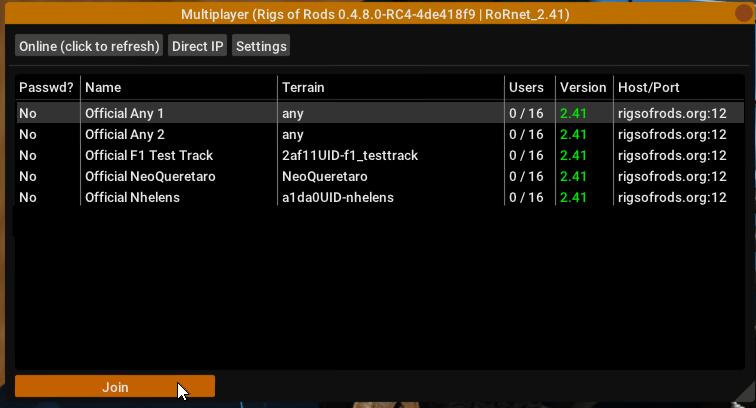
\includegraphics{images/bg-mp3.png}
The `any' servers allow you to select a terrain, while other servers
(such as Official Nhelens) are set to use a specific terrain.
While on a server, you can enable collisions between other players or
hide nicknames by going to \texttt{Settings} in the top menubar.

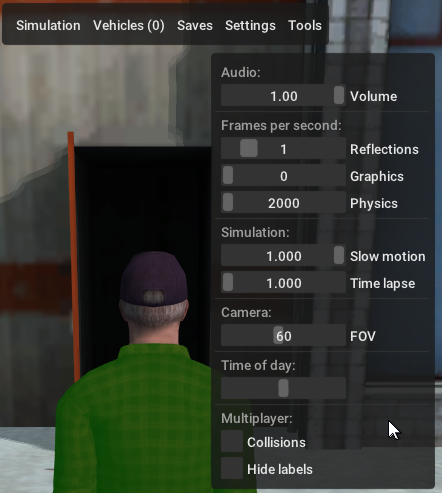
\includegraphics{images/bg-mp4.png}

Note that multiplayer is still in development and can be unstable at
times!

\hypertarget{controls-config}{%
\chapter{Controls and configuration}\label{controls-config}}

\hypertarget{intro}{%
\section{Intro}\label{intro}}

Rigs of Rods is a simulator which strives for maximum reallism, and
hence you need an appropriate controller, such as a wheel for land
vehicles and joystick for aerial or marine vehicles.

Input is configured by editing configuration file
\protect\hyperlink{config-file-inputmap}{input.map} or by using the
\protect\hyperlink{configuring-controls-with-the-input-mapping-tool}{Input
Mapping Tool}. In-game configuration of controls is not implemented yet.

\hypertarget{keyboard-layout}{%
\section{Keyboard layout}\label{keyboard-layout}}

\hypertarget{general-controls}{%
\subsection{General controls}\label{general-controls}}

\begin{tabular}{ |l|l| } 
\hline
\textbf{General} & \textbf{Key} \\
\hline
Pause game & ESC \\
\hline
Quit game & ALT+F4 \\
\hline
Spawn new vehicle & CTRL+G \\
\hline
Enter or exit vehicle & ENTER \\
\hline
Reset vehicle & I \\
\hline
Reset vehicle in place & BACKSPACE \\
\hline
View vehicle statistics & T \\
\hline
View vehicle commands & CTRL+T \\
\hline
Screenshot & Print Screen/SYSRQ \\
\hline
Chat (Multiplayer) & Y \\
\hline
Toggle HUD & U \\
\hline
Toggle soft reset mode & APOSTROPHE \\
\hline
Toggle limited camera movement & SHIFT+SPACE \\
\hline
Adjust simulation speed & CTRL+= / SHIFT+= \\
\hline
Reset simulation speed/set preset & BACKSLASH \\
\hline
Switch between vehicles & CTRL+RBRACKET / CTRL+LBRACKET  \\
\hline
Remove current vehicle & CTRL+Del \\
\hline
Respawn last vehicle & CTRL+ . (period) \\
\hline
\end{tabular}

\hypertarget{character}{%
\subsubsection{Character}\label{character}}
\begin{tabular}{ |l|l| } 
\hline
Character & Key \\
\hline
Jump & SPACE \\
\hline
Turn right & RIGHT \\
\hline
Turn left & LEFT \\
\hline
Walk forwards & UP \\
\hline
Walk backwards & DOWN \\
\hline
Run & SHIFT+UP \\
\hline
\end{tabular}

\hypertarget{camera}{%
\subsubsection{Camera}\label{camera}}

\begin{tabular}{ |l|l| } 
\hline
Camera & Key \\
\hline
Change view & C \\
\hline
Rotate up/down & Numpad 8 / Numpad 2 \\
\hline
Rotate left/right & Numpad 4 / Numpad 6 \\
\hline
Zoom in/out & Numpad 9 / Numpad 3 \\
\hline
Zoom in/out (fast) & SHIFT+Numpad 9 / SHIFT+Numpad 3 \\
\hline
Free camera & SHIFT+C \\
\hline
Fixed camera & ALT+C \\
\hline
\end{tabular}

\hypertarget{time}{%
\subsubsection{Time}\label{time}}

(Sky type must be set to Caelum or SkyX)

\begin{tabular}{ |l|l| } 
\hline
Time Adjust & Key \\
\hline
Change time & Numpad + (plus) / Numpad - (minus) \\
\hline
Change time (fast) & SHIFT+Numpad + (plus) / SHIFT+Numpad - (minus) \\
\hline
\end{tabular}

\hypertarget{overview-map}{%
\subsubsection{Overview map}\label{overview-map}}

\begin{tabular}{ |l|l| } 
\hline
Map & Key \\
\hline
Toggle map view & TAB \\
\hline
Zoom in/out & CTRL+TAB / SHIFT+TAB \\
\hline
Toggle alpha & CTRL+SHIFT+TAB \\
\hline
Toggle icons & CTRL+SHIFT+ALT+TAB \\
\hline
\end{tabular}

\hypertarget{saves}{%
\subsubsection{Saves}\label{saves}}

\begin{tabular}{ |l|l| } 
\hline
Savegames & Key \\
\hline
Quick save & NUMPAD / (divide) \\
\hline
Quick load & NUMPAD * (multiply) \\
\hline
Save slot 1 & CTRL+ALT+1 \\
\hline
Save slot 2 & CTRL+ALT+2 \\
\hline
Save slot 3 & CTRL+ALT+3 \\
\hline
Save slot 4 & CTRL+ALT+4 \\
\hline
Save slot 5 & CTRL+ALT+5 \\
\hline
Load slot 1 & ALT+1 \\
\hline
Load slot 2 & ALT+2 \\
\hline
Load slot 3 & ALT+3 \\
\hline
Load slot 4 & ALT+4 \\
\hline
Load slot 5 & ALT+5 \\
\hline
\end{tabular}

Note: You can load a savegame from the main menu.

\hypertarget{common-vehicle-controls}{%
\subsection{Common vehicle controls}\label{common-vehicle-controls}}

\begin{tabular}{ |l|l| } 
\hline
Basic vehicle controls & Key \\
\hline
Steer Left & LEFT \\
\hline
Steer Right & RIGHT \\
\hline
Accelerate/Brake & UP / DOWN \\
\hline
\end{tabular}

\hypertarget{shifting}{%
\subsubsection{Shifting}\label{shifting}}

\begin{tabular}{ |l|l| } 
\hline
Shifting & Key \\
\hline
Autoshift up & PGUP \\
\hline
Autoshift down & PGDOWN \\
\hline
Switch shift modes & Q \\
\hline
Manual clutch & SHIFT \\
\hline
Shift up & A \\
\hline
Shift down & Z \\
\hline
\end{tabular}


\hypertarget{misc}{%
\subsubsection{Misc}\label{misc}}

\begin{tabular}{ |l|l| } 
\hline
Misc & Key \\
\hline
Truck horn & H \\
\hline
Parking brake & P \\
\hline
Trailer parking brake & CTRL+P \\
\hline
Blinker left & COMMA \\
\hline
Blinker right & DOT \\
\hline
Blinker warn & PERIOD \\
\hline
Toggle contact & X \\
\hline
Starter (hold) & S \\
\hline
Attach trailer & L \\
\hline
Inter-wheel differentals & W \\
\hline
Inter-axle differentals & CTRL+W \\
\hline
Transfer case (2WD/4WD) & SHIFT+W \\
\hline
Alternate gear ratios & ALT+W \\
\hline
Secure Load & O \\
\hline
Show skeleton & K \\
\hline
Cycle skeleton views & CTRL+K \\
\hline
Toggle lights & N \\
\hline
Toggle beacons & M \\
\hline
Rescue truck & R \\
\hline
Particle cannon & G \\
\hline
Tire Pressure(not for all trucks) & RBRACKET {[} / LBRACKET {]} \\
\hline
\end{tabular}

\hypertarget{commands}{%
\subsubsection{Commands}\label{commands}}

\begin{tabular}{ |l|l| } 
\hline
Function keys & Combo \\
\hline
COMMANDS 01 & F1 \\
\hline
\ldots{} & \ldots{} \\
\hline
COMMANDS 12 & F12 \\
\hline
COMMANDS 13 & CTRL + F1 \\
\hline
\ldots{} & \ldots{} \\
\hline
COMMANDS 24 & CTRL + F12 \\
\hline
COMMANDS 25 & ALT + F1 \\
\hline
\ldots{} & \ldots{} \\
\hline
COMMANDS 36 & ALT + F12 \\
\hline
COMMANDS 37 & CTRL + ALT + F1 \\
\hline
\ldots{} & \ldots{} \\
\hline
COMMANDS 48 & CTRL + ALT + F12 \\
\hline
COMMANDS 49 & CTRL+ SHIFT + F1 \\
\hline
\ldots{} & \ldots{} \\
\hline
COMMANDS 58 & CTRL + SHIFT + F10 \\
\hline
COMMANDS 59 & CTRL + SHIFT + F11 \\
\hline
\ldots{} & \ldots{} \\
\hline
COMMANDS 68 & CTRL + ALT + F8 \\
\hline
COMMANDS 69 & CTRL + ALT + F9 \\
\hline
\ldots{} & \ldots{} \\
\hline
COMMANDS 78 & CTRL + SHIFT + ALT + F6 \\
\hline
COMMANDS 79 & CTRL + SHIFT + ALT + F7 \\
\hline
\ldots{} & \ldots{} \\
\hline
COMMANDS 83 & CTRL + SHIFT + ALT + F11 \\
\hline
COMMANDS 84 & CTRL + SHIFT + ALT + F12 \\
\hline
\end{tabular}

\hypertarget{aerial-and-marine-controls}{%
\subsection{Aerial and marine
controls}\label{aerial-and-marine-controls}}


\hypertarget{planes}{%
\subsubsection{Planes}\label{planes}}

\begin{tabular}{ |l|l| } 
\hline
Airplane controls & Key \\
\hline
Steer left & LEFT \\
\hline
Steer right & RIGHT \\
\hline
Elevator up & UP \\
\hline
Elevator down & DOWN \\
\hline
Rudder right & X \\
\hline
Rudder left & Z \\
\hline
Brake & B \\
\hline
Parking brake & P \\
\hline
Reverse & R \\
\hline
Less flaps & 1 \\
\hline
More flaps & 2 \\
\hline
Less airbrakes & 3 \\
\hline
More airbrakes & 4 \\
\hline
Throttle down & PAGE-DOWN \\
\hline
Throttle up & PAGE-UP \\
\hline
Start engines & CLICK BUTTONS ``ON'' \\
\hline
Start all engines & CTRL+HOME \\
\hline
Full throttle & CTRL+PAGEUP \\
\hline
No throttle & CTRL+PAGEDOWN \\
\hline
\end{tabular}

It is recommended to use: \texttt{CTRL+Home} to start all engines of a
plane and \texttt{CTRL+PAGE-UP} to full throttle all engines because
some planes could have more than 4 engines and you couldn't control them
with your mouse.

\hypertarget{boats}{%
\subsubsection{Boats}\label{boats}}

\begin{tabular}{ |l|l| } 
\hline
Boat controls & Key \\
\hline
Throttle down & DOWN \\
\hline
Throttle up & UP \\
\hline
Steer left & LEFT \\
\hline
Steer right & RIGHT \\
\hline
Center rudder & PGUP \\
\hline
Center throttle & PGDOWN \\
\hline
\end{tabular}

\hypertarget{config-file-input.map}{%
\section{Config file `input.map'}\label{config-file-input.map}}

For all keys, see the
\href{https://github.com/RigsOfRods/rigs-of-rods/blob/master/resources/skeleton/config/input.map}{input.map}
file on GitHub.

This file defines all key alias for RoR. It has the following format:

\begin{verbatim}
EVENT_NAME    EVENT_TYPE    MAPPING
\end{verbatim}

For example:

\begin{verbatim}
BOAT_CENTER_RUDDER     Keyboard    DOWN
\end{verbatim}

This binds the BOAT\_CENTER\_RUDDER event to the Down arrow on your
keyboard.

A list of all valid events can be found in the
\protect\hyperlink{keypress-events}{Keypress Events} section.

\hypertarget{keyboard}{%
\subsection{Keyboard}\label{keyboard}}

For the keyboard there are several special things:

\hypertarget{modifiers}{%
\subsubsection{Modifiers}\label{modifiers}}

\begin{itemize}
\tightlist
\item
  CTRL
\item
  SHIFT
\item
  ALT
\end{itemize}

Combine them with a + sign. Example:

\begin{verbatim}
CAMERA_FREE_MODE    Keyboard    EXPL+SHIFT+C
\end{verbatim}

\hypertarget{the-expl-tag}{%
\subsubsection{The EXPL tag}\label{the-expl-tag}}

A special keyword used in defining commands.

In this example, only COMMANDS\_01 is triggered when pressing F1, and
COMMANDS\_13 is triggered when pressing CTRL+F1 (but not COMMANDS\_01)

\begin{verbatim}
COMMANDS_01                    Keyboard             EXPL+F1 
COMMANDS_13                    Keyboard             EXPL+CTRL+F1 
\end{verbatim}

In this example, COMMANDS\_01 would be triggered if you press CTRL+F1,
as F1 is part of the COMMANDS\_13 combination.

\begin{verbatim}
COMMANDS_01                    Keyboard             F1 
COMMANDS_13                    Keyboard             CTRL+F1 
\end{verbatim}

\newpage
\hypertarget{list-of-usable-keys}{%
\subsubsection{List of usable keys}\label{list-of-usable-keys}}

\begin{verbatim}
0
1
2
3
4
5
6
7
8
9
A
ABNT_C1
ABNT_C2
ADD
APOSTROPHE
APPS
AT
AX
B
BACK
BACKSLASH
C
CALCULATOR
CAPITAL
COLON
COMMA
CONVERT
D
DECIMAL
DELETE
DIVIDE
DOWN
E
END
EQUALS
ESCAPE
F
F1
F10
F11
F12
F13
F14
F15
F2
F3
F4
F5
F6
F7
F8
F9
G
GRAVE
H
HOME
I
INSERT
J
K
KANA
KANJI
L
LBRACKET
LCONTROL
LEFT
LMENU
LSHIFT
LWIN
M
MAIL
MEDIASELECT
MEDIASTOP
MINUS
MULTIPLY
MUTE
MYCOMPUTER
N
NEXTTRACK
NOCONVERT
NUMLOCK
NUMPAD0
NUMPAD1
NUMPAD2
NUMPAD3
NUMPAD4
NUMPAD5
NUMPAD6
NUMPAD7
NUMPAD8
NUMPAD9
NUMPADCOMMA
NUMPADENTER
NUMPADEQUALS
O
OEM_102
P
PAUSE
PERIOD
PGDOWN
PGUP
PLAYPAUSE
POWER
PREVTRACK
Q
R
RBRACKET
RCONTROL
RETURN
RIGHT
RMENU
RSHIFT
RWIN
S
SCROLL
SEMICOLON
SLASH
SLEEP
SPACE
STOP
SUBTRACT
SYSRQ
T
TAB
U
UNDERLINE
UNLABELED
UP
V
VOLUMEDOWN
VOLUMEUP
W
WAKE
WEBBACK
WEBFAVORITES
WEBFORWARD
WEBHOME
WEBREFRESH
WEBSEARCH
WEBSTOP
X
Y
YEN
Z
\end{verbatim}

\hypertarget{joystick-wheel-or-gamepad}{%
\subsection{Joystick, Wheel or
gamepad}\label{joystick-wheel-or-gamepad}}

This category covers all analogue input devices detected by the
operating system, so all gamepads, joysticks, wheels, pedals, etc.

\hypertarget{joystickbutton}{%
\subsubsection{JoystickButton}\label{joystickbutton}}

Arguments:

\begin{itemize}
\tightlist
\item
  Joystick Number (unused in modern mappings), set to 0
\item
  Button number
\end{itemize}

\begin{verbatim}
AIRPLANE_THROTTLE_DOWN    JoystickButton    0    2
\end{verbatim}

\hypertarget{joystickaxis}{%
\subsubsection{JoystickAxis}\label{joystickaxis}}

Arguments:

\begin{itemize}
\tightlist
\item
  Joystick Number (unused in modern mappings), set to 0
\item
  Axis number
\item
  Options:

  \begin{itemize}
  \tightlist
  \item
    HALF
  \item
    REVERSE
  \item
    UPPER
  \item
    LOWER
  \item
    RELATIVE
  \item
    DIGITAL
  \item
    DEADZONE : add deadzone in percent with equal sign:
    ``DEADZONE=0.15''.
  \item
    LINEARITY: add linearity in percent with equal sign:
    ``LINEARITY=0.15''.
  \end{itemize}
\end{itemize}

\begin{verbatim}
AIRPLANE_STEER_RIGHT    JoystickAxis    0    1    UPPER+DEADZONE = 0.15
\end{verbatim}

\hypertarget{joystickpov}{%
\subsubsection{JoystickPov}\label{joystickpov}}

Arguments:

\begin{itemize}
\tightlist
\item
  Joystick Number (unused in modern mappings), set to 0
\item
  POV number
\item
  Direction: North, South, East, West, NorthEast, SouthEast, NorthWest,
  SouthWest.
\end{itemize}

\begin{verbatim}
CHARACTER_FORWARD    JoystickPov    0    0    North
\end{verbatim}

\hypertarget{joystickslider-joysticksliderx-joystickslidery}{%
\subsubsection{JoystickSlider, JoystickSliderX,
JoystickSliderY}\label{joystickslider-joysticksliderx-joystickslidery}}

Arguments:

\begin{itemize}
\tightlist
\item
  Joystick Number (unused in modern mappings), set to 0
\item
  Slider number
\item
  Options:

  \begin{itemize}
  \tightlist
  \item
    REVERSE
  \end{itemize}
\end{itemize}

\begin{verbatim}
TRUCK_MANUAL_CLUTCH    JoystickSliderY    0    Y    0    REVERSE+DEADZONE = -30
\end{verbatim}

\hypertarget{keypress-events}{%
\section{Keypress Events}\label{keypress-events}}

\textbf{Keypress event identification in RoR 0.4.7.0+}

These are all the valid keypress events, they can be used in a input map
or for
\href{http://docs.rigsofrods.org/vehicle-creation/fileformat-truck/\#add_animation}{prop
animations}. not all make sense though for animated props.

\begin{verbatim}
AIRPLANE_AIRBRAKES_FULL     
AIRPLANE_AIRBRAKES_LESS     
AIRPLANE_AIRBRAKES_MORE     
AIRPLANE_AIRBRAKES_NONE     
AIRPLANE_BRAKE              
AIRPLANE_ELEVATOR_DOWN      
AIRPLANE_ELEVATOR_UP        
AIRPLANE_FLAPS_FULL         
AIRPLANE_FLAPS_LESS         
AIRPLANE_FLAPS_MORE         
AIRPLANE_FLAPS_NONE         
AIRPLANE_PARKING_BRAKE      
AIRPLANE_REVERSE            
AIRPLANE_RUDDER_LEFT        
AIRPLANE_RUDDER_RIGHT       
AIRPLANE_STEER_LEFT         
AIRPLANE_STEER_RIGHT        
AIRPLANE_THROTTLE_AXIS      
AIRPLANE_THROTTLE_DOWN      
AIRPLANE_THROTTLE_FULL      
AIRPLANE_THROTTLE_NO        
AIRPLANE_THROTTLE_UP        
AIRPLANE_TOGGLE_ENGINES     
BOAT_CENTER_RUDDER          
BOAT_REVERSE                
BOAT_STEER_LEFT             
BOAT_STEER_RIGHT            
BOAT_THROTTLE_AXIS          
BOAT_THROTTLE_UP            
BOAT_THROTTLE_DOWN          
CAMERA_CHANGE               
CAMERA_FREE_MODE            
CAMERA_FREE_MODE_FIX        
CAMERA_LOOKBACK             
CAMERA_RESET                
CAMERA_UP                   
CAMERA_DOWN                 
CAMERA_ROTATE_DOWN          
CAMERA_ROTATE_LEFT          
CAMERA_ROTATE_RIGHT         
CAMERA_ROTATE_UP            
CAMERA_ZOOM_IN              
CAMERA_ZOOM_IN_FAST         
CAMERA_ZOOM_OUT             
CAMERA_ZOOM_OUT_FAST        
SKY_DECREASE_TIME           
SKY_DECREASE_TIME_FAST      
SKY_INCREASE_TIME           
SKY_INCREASE_TIME_FAST      
CHARACTER_BACKWARDS         
CHARACTER_FORWARD           
CHARACTER_JUMP              
CHARACTER_LEFT              
CHARACTER_RIGHT             
CHARACTER_ROT_DOWN          
CHARACTER_ROT_UP            
CHARACTER_RUN               
CHARACTER_RUN               
CHARACTER_SIDESTEP_LEFT     
CHARACTER_SIDESTEP_RIGHT    
COMMANDS_01                 
COMMANDS_02                 
COMMANDS_03                 
COMMANDS_04                 
COMMANDS_05                 
COMMANDS_06                 
COMMANDS_07                 
COMMANDS_08                 
COMMANDS_09                 
COMMANDS_10                 
COMMANDS_11                 
COMMANDS_12                 
COMMANDS_13                 
COMMANDS_14                 
COMMANDS_15                 
COMMANDS_16                 
COMMANDS_17                 
COMMANDS_18                 
COMMANDS_19                 
COMMANDS_20                 
COMMANDS_21                 
COMMANDS_22                 
COMMANDS_23                 
COMMANDS_24                 
COMMANDS_25                 
COMMANDS_26                 
COMMANDS_27                 
COMMANDS_28                 
COMMANDS_29                 
COMMANDS_30                 
COMMANDS_31                 
COMMANDS_32                 
COMMANDS_33                 
COMMANDS_34                 
COMMANDS_35                 
COMMANDS_36                 
COMMANDS_37                 
COMMANDS_38                 
COMMANDS_39                 
COMMANDS_40                 
COMMANDS_41                 
COMMANDS_42                 
COMMANDS_43                 
COMMANDS_44                 
COMMANDS_45                 
COMMANDS_46                 
COMMANDS_47                 
COMMANDS_48                 
COMMANDS_49                 
COMMANDS_50                 
COMMANDS_51                 
COMMANDS_52                 
COMMANDS_53                 
COMMANDS_54                 
COMMANDS_55                 
COMMANDS_56                 
COMMANDS_57                 
COMMANDS_58                 
COMMANDS_59                 
COMMANDS_60                 
COMMANDS_61                 
COMMANDS_62                 
COMMANDS_63                 
COMMANDS_64                 
COMMANDS_65                 
COMMANDS_66                 
COMMANDS_67                 
COMMANDS_68                 
COMMANDS_69                 
COMMANDS_70                 
COMMANDS_71                 
COMMANDS_72                 
COMMANDS_73                 
COMMANDS_74                 
COMMANDS_75                 
COMMANDS_76                 
COMMANDS_77                 
COMMANDS_78                 
COMMANDS_79                 
COMMANDS_80                 
COMMANDS_81                 
COMMANDS_82                 
COMMANDS_83                 
COMMANDS_84                 
COMMON_ACCELERATE_SIMULATION
COMMON_DECELERATE_SIMULATION
COMMON_RESET_SIMULATION_PACE
COMMON_CONSOLE_TOGGLE       
COMMON_ENTER_OR_EXIT_TRUCK  
COMMON_ENTER_NEXT_TRUCK     
COMMON_ENTER_PREVIOUS_TRUCK 
COMMON_REMOVE_CURRENT_TRUCK 
COMMON_RESPAWN_LAST_TRUCK   
COMMON_FULLSCREEN_TOGGLE    
COMMON_HIDE_GUI             
COMMON_LOCK                 
COMMON_AUTOLOCK             
COMMON_ROPELOCK             
COMMON_OUTPUT_POSITION      
COMMON_GET_NEW_VEHICLE      
COMMON_PRESSURE_LESS        
COMMON_PRESSURE_MORE        
COMMON_QUIT_GAME            
COMMON_REPLAY_BACKWARD      
COMMON_REPLAY_FAST_BACKWARD 
COMMON_REPLAY_FAST_FORWARD  
COMMON_REPLAY_FORWARD       
COMMON_RESCUE_TRUCK         
COMMON_RESET_TRUCK          
COMMON_SCREENSHOT           
COMMON_SECURE_LOAD          
COMMON_SHOW_SKELETON        
COMMON_TOGGLE_TERRAIN_EDITOR
COMMON_TOGGLE_CUSTOM_PARTICL
COMMON_TOGGLE_MAT_DEBUG     
COMMON_TOGGLE_RENDER_MODE   
COMMON_TOGGLE_REPLAY_MODE   
COMMON_TOGGLE_STATS         
COMMON_TOGGLE_TRUCK_BEACONS 
COMMON_TOGGLE_TRUCK_LIGHTS  
COMMON_TRUCK_INFO           
COMMON_TRUCK_DESCRIPTION    
COMMON_FOV_LESS             
COMMON_FOV_MORE             
GRASS_LESS                  
GRASS_MORE                  
GRASS_MOST                  
GRASS_NONE                  
GRASS_SAVE                  
SURVEY_MAP_ZOOM_IN          
SURVEY_MAP_ZOOM_OUT         
SURVEY_MAP_TOGGLE_VIEW      
SURVEY_MAP_TOGGLE_ALPHA     
SURVEY_MAP_TOGGLE_ICONS     
MENU_DOWN                   
MENU_LEFT                   
MENU_RIGHT                  
MENU_SELECT                 
MENU_UP                     
TRUCK_ACCELERATE            
TRUCK_ACCELERATE_MODIFIER_25
TRUCK_ACCELERATE_MODIFIER_50
TRUCK_ANTILOCK_BRAKE        
TRUCK_AUTOSHIFT_DOWN        
TRUCK_AUTOSHIFT_UP          
TRUCK_BLINK_LEFT            
TRUCK_BLINK_RIGHT           
TRUCK_BLINK_WARN            
TRUCK_BRAKE                 
TRUCK_BRAKE_MODIFIER_25     
TRUCK_BRAKE_MODIFIER_50     
TRUCK_CRUISE_CONTROL        
TRUCK_CRUISE_CONTROL_READJUS
TRUCK_CRUISE_CONTROL_ACCL   
TRUCK_CRUISE_CONTROL_DECL   
TRUCK_HORN                  
TRUCK_LIGHTTOGGLE1          
TRUCK_LIGHTTOGGLE2          
TRUCK_LIGHTTOGGLE3          
TRUCK_LIGHTTOGGLE4          
TRUCK_LIGHTTOGGLE5          
TRUCK_LIGHTTOGGLE6          
TRUCK_LIGHTTOGGLE7          
TRUCK_LIGHTTOGGLE8          
TRUCK_LIGHTTOGGLE9          
TRUCK_LIGHTTOGGLE10         
TRUCK_MANUAL_CLUTCH         
TRUCK_PARKING_BRAKE         
TRUCK_SHIFT_DOWN            
TRUCK_SHIFT_NEUTRAL         
TRUCK_SHIFT_UP              
TRUCK_STARTER               
TRUCK_STEER_LEFT            
TRUCK_STEER_RIGHT           
TRUCK_SWITCH_SHIFT_MODES    
TRUCK_TOGGLE_AXLE_LOCK      
TRUCK_TOGGLE_CONTACT        
TRUCK_TOGGLE_FORWARDCOMMANDS
TRUCK_TOGGLE_IMPORTCOMMANDS 
TRUCK_TOGGLE_VIDEOCAMERA    
TRUCK_TRACTION_CONTROL      
\end{verbatim}

\hypertarget{mouse}{%
\section{Mouse}\label{mouse}}

\hypertarget{required-applications}{%
\subsubsection{Required applications}\label{required-applications}}

\href{http://vjoystick.sourceforge.net/site/index.php/download-a-install/72-download}{vJoy
joystick emulator}

\href{http://andersmalmgren.github.io/FreePIE/index.html}{FreePIE input
emulator}

\hypertarget{setting-up-the-input-map-and-freepie-script}{%
\subsubsection{Setting up the input map and FreePIE
script}\label{setting-up-the-input-map-and-freepie-script}}

After installing the above applications, download
\href{/download/RoR_Mouse_Control.zip}{this zip file} which contains the
required input map and FreePIE script.

There will be two files in the zip: \texttt{vJoy\_Device.map} and
\texttt{MouseControl.py}.

Extract both files into
\texttt{Documents\textbackslash{}Rigs\ of\ Rods\ 0.4\textbackslash{}config}.

\hypertarget{using-freepie}{%
\subsubsection{Using FreePIE}\label{using-freepie}}

Open FreePIE and press \texttt{File\ -\textgreater{}\ Open}. Browse to
the \texttt{MouseControl.py} file you downloaded earlier:

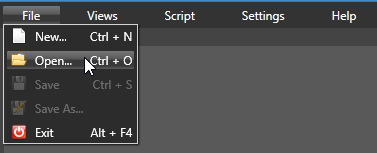
\includegraphics{images/FreePIE-1.png}

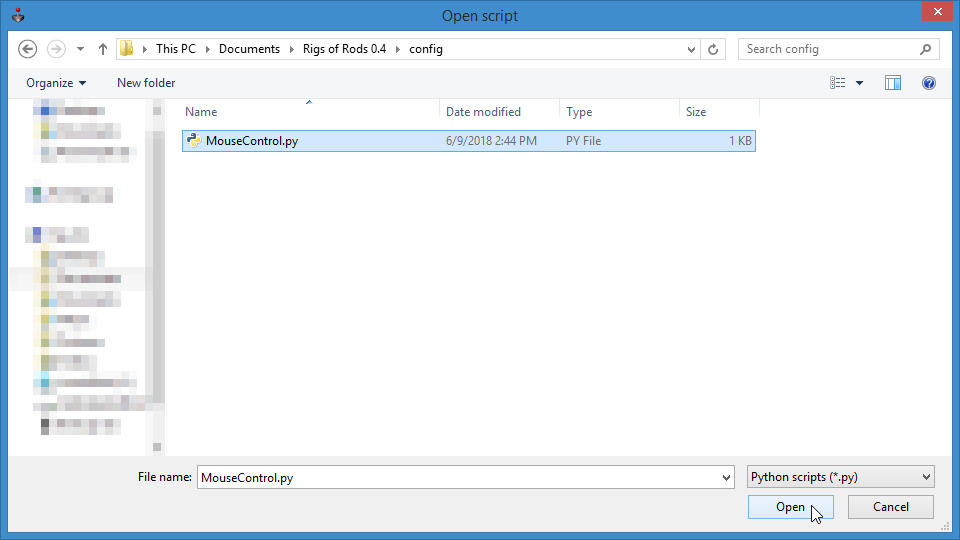
\includegraphics{images/FreePIE-2.png}

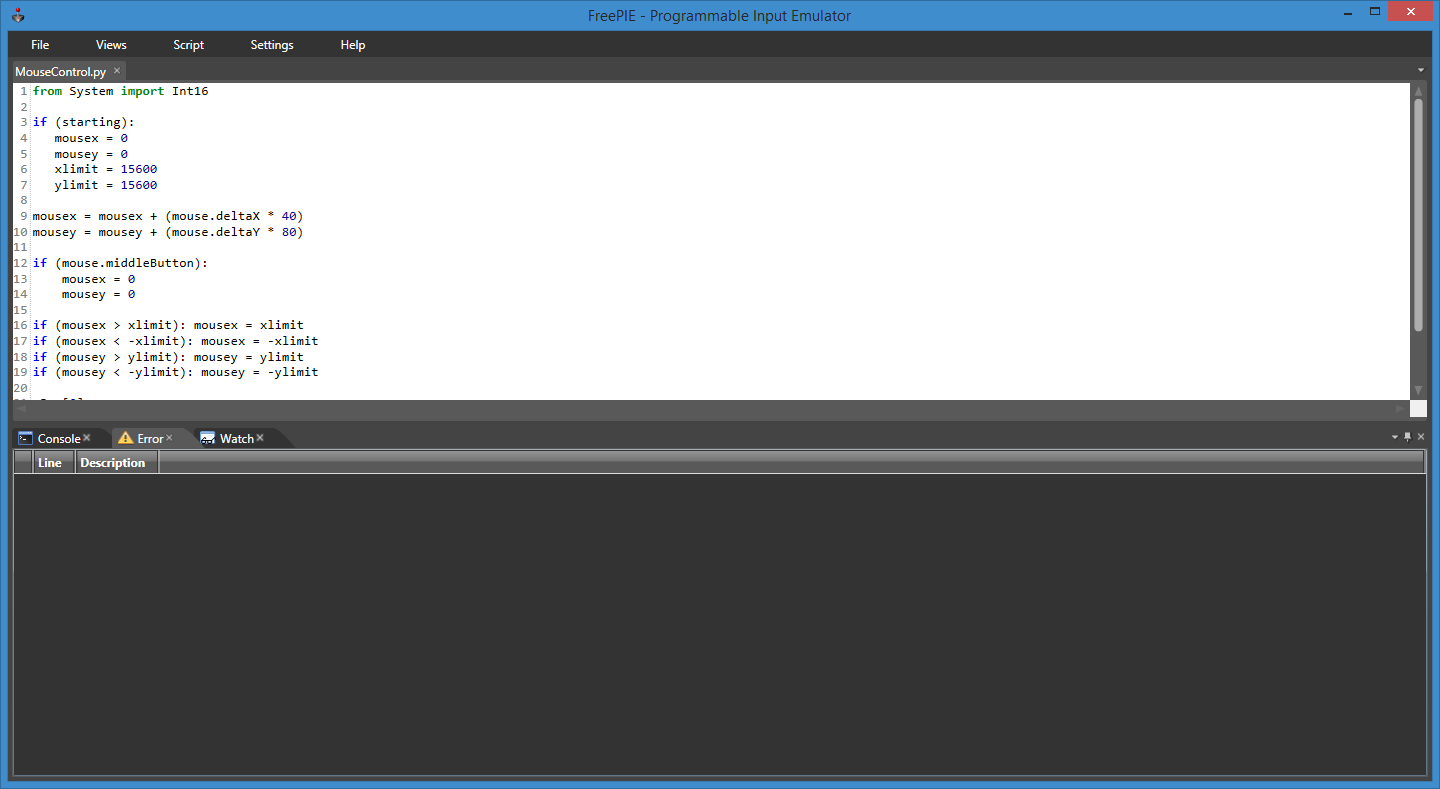
\includegraphics{images/FreePIE-3.png}

Then press \texttt{Script\ -\textgreater{}\ Run\ script}:

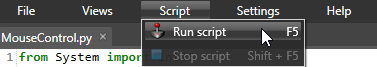
\includegraphics{images/FreePIE-4.png}


The script should now be running. If you get an error, install vJoy.

Leave FreePIE running, launch RoR and you should now have mouse control!

You can modify both the script and the input map to make them better
suit for your use.

For example the numbers \texttt{40} and \texttt{80} in the script are
the sensitivity of the controls.

Mouse middle button in the script above, will reset the axises in game,
in this case the steering and throttle.

\hypertarget{configuring-controls-with-the-input-mapping-tool}{%
\section{Configuring controls with the Input Mapping
Tool}\label{configuring-controls-with-the-input-mapping-tool}}

The easiest way to configure your device for use in Rigs of Rods is to
use the
\href{https://forum.rigsofrods.org/resources/windows-input-mapping-tool.13/}{Input
Mapping Tool}.

\hypertarget{vjoy-conflicts}{%
\subsection{vJoy Conflicts}\label{vjoy-conflicts}}

\textbf{NOTE: If you have vJoy installed, you will have to disable it
before running the tool!}

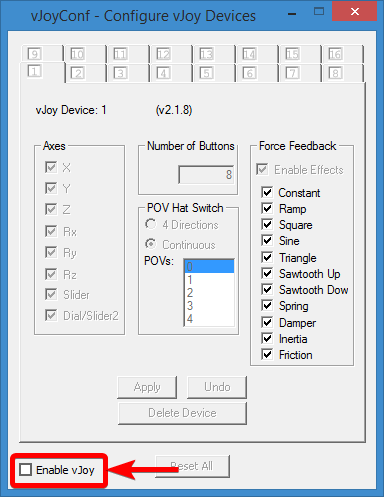
\includegraphics{images/vJoyDisable.png}

\hypertarget{launching-the-tool}{%
\subsection{Launching the tool}\label{launching-the-tool}}

After downloading, extract the zip into a new folder. Then double-click
\texttt{Run.bat} to launch the tool.

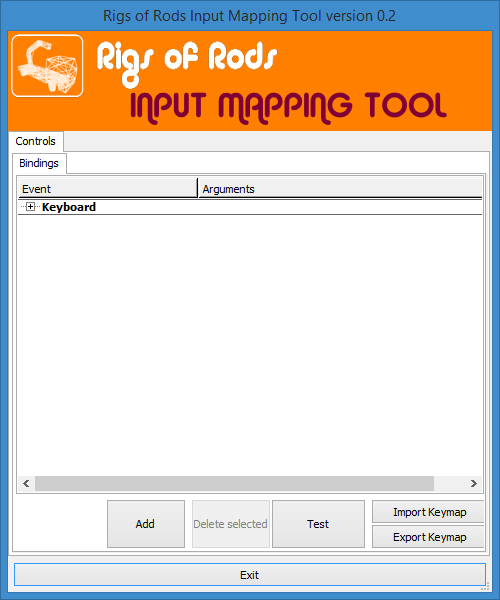
\includegraphics{images/InputMappingTool-1.png}

\hypertarget{adding-new-inputs}{%
\subsection{Adding new inputs}\label{adding-new-inputs}}

To begin adding inputs, click \texttt{Add}.

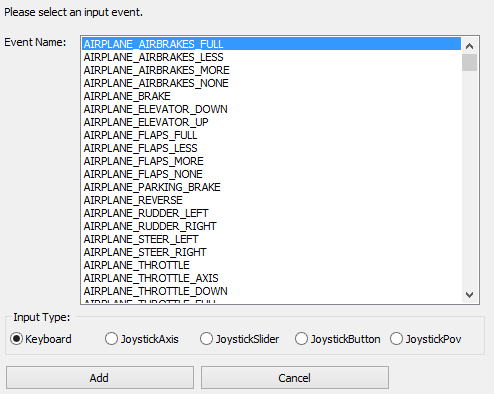
\includegraphics{images/InputMappingTool-2.png}

Select the event you want to assign an input to. In this exanmple, I
will use \texttt{TRUCK\_ACCELERATE}

Then select the correct input type:

Event type

Description

Keyboard

All keys on the keyboard.

JoystickAxis

Used for steering wheels/sticks/etc.

JoystickSlider

Any type of slider, mainly seen on flight sticks.

JoystickButton

Buttons! (e.g.~\texttt{A} button on an Xbox controller)

JoystickPov

Used for D-Pad controls.

Click \texttt{Add} once ready, the tool will then ask you to move the
axis/press a button.

The popup will automatically close once the requested action is
completed.

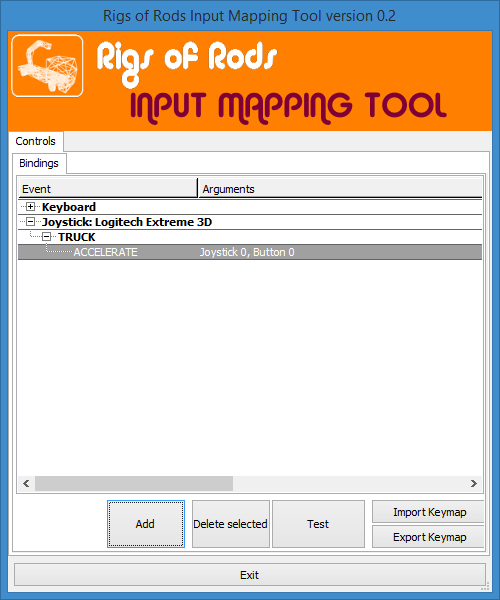
\includegraphics{images/InputMappingTool-3.png}

Repeat the process for all the inputs you want to add.

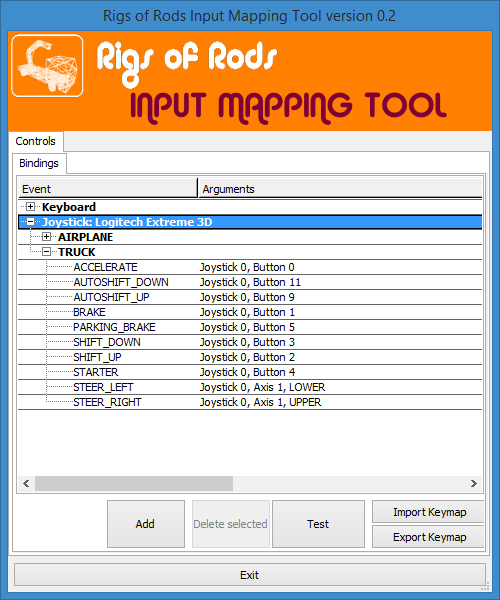
\includegraphics{images/InputMappingTool-4.png}

Once you're done, it's time to export the keymap.

\hypertarget{exporting-the-keymap}{%
\subsection{Exporting the keymap}\label{exporting-the-keymap}}

First, you'll need to get the correct file name of your file.

To do this, double-click \texttt{getdeviceinfo.exe}. This will generate
a \texttt{inputinfo.txt} file. Open the text file.

Example output:

\begin{verbatim}
System info:
    OIS Version: 1.3.0
    OIS Release Name: 1.3.0
    Input Manager: Win32InputManager
    Total Keyboards: 1
    Total Mice: 1
    Total JoySticks: 1

Devices:
    - OISKeyboard, Vendor: Win32InputManager
    - OISMouse, Vendor: Win32InputManager
    - OISJoyStick, Vendor: Logitech Extreme 3D


Joystick 0:
    Vendor: Logitech Extreme 3D
    VendorMapFilename: Logitech_Extreme_3D.map
    ID: 0
    Type: [3] OISJoyStick
    Axes: 3
    Sliders: 1
    POV/HATs: 1
    Buttons: 12
    Vector3: 0
    Vector3Sensitivity: 2.28
\end{verbatim}

\texttt{VendorMapFilename} will be the name of your exported file. In
this example, the name will be \texttt{Logitech\_Extreme\_3D.map}.

Click \texttt{Export\ Keymap} then select your device from the list.

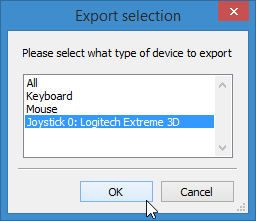
\includegraphics{images/InputMappingTool-5.png}

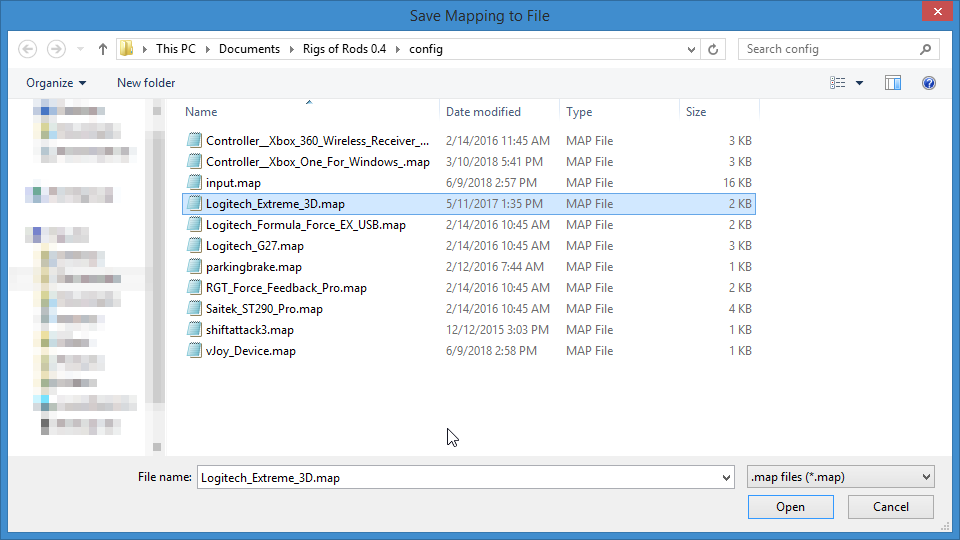
\includegraphics{images/InputMappingTool-6.png}

And finally, run Rigs of Rods and test your device! You can make further
edits to your input map by clicking \texttt{Import\ Keymap}.

If you want to share your created input map, upload it to the
Miscellaneous section of the
\href{https://forum.rigsofrods.org/resources/}{Repository}. Thanks!


\hypertarget{installing-content}{%
\chapter{Installing content}\label{installing-content}}

This page will show you how to install vehicles and terrains for Rigs of
Rods.

\hypertarget{installing-mods-from-the-repository}{%
\section{Installing mods from the
Repository}\label{installing-mods-from-the-repository}}

\hypertarget{downloading}{%
\subsection{Downloading}\label{downloading}}

Visit the \href{https://forum.rigsofrods.org/resources/}{Repository}.

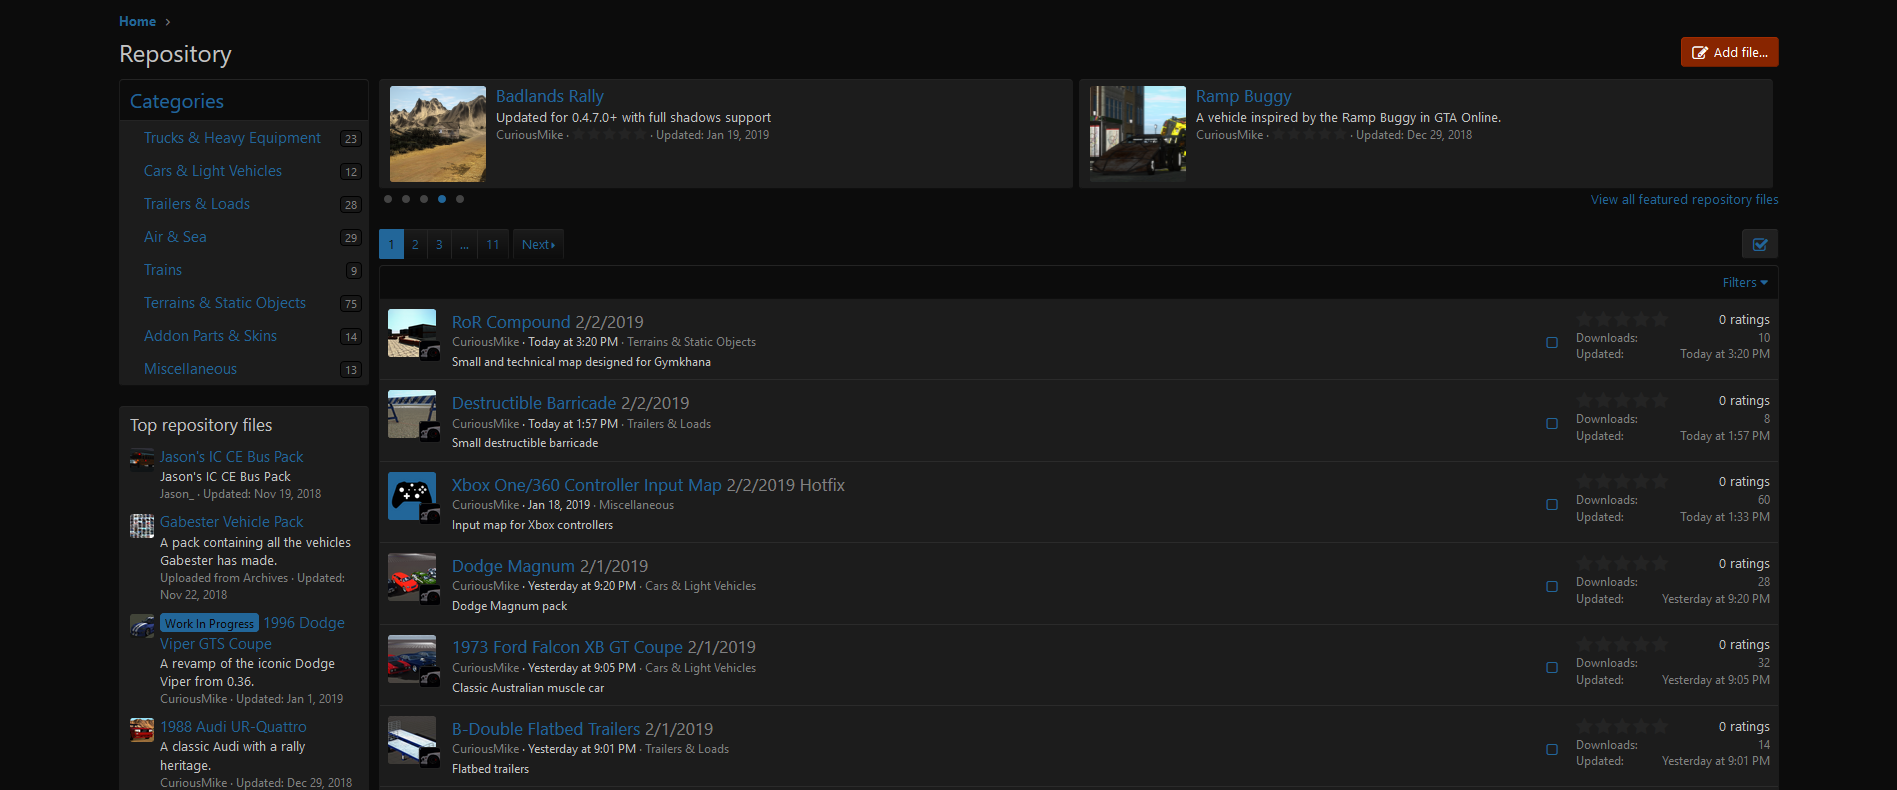
\includegraphics{images/repository.png}

Find something you like. For example, how about the nice
\href{https://forum.rigsofrods.org/resources/1996-dodge-viper-gts-coupe.88/}{1996
Dodge Viper GTS Coupe}:

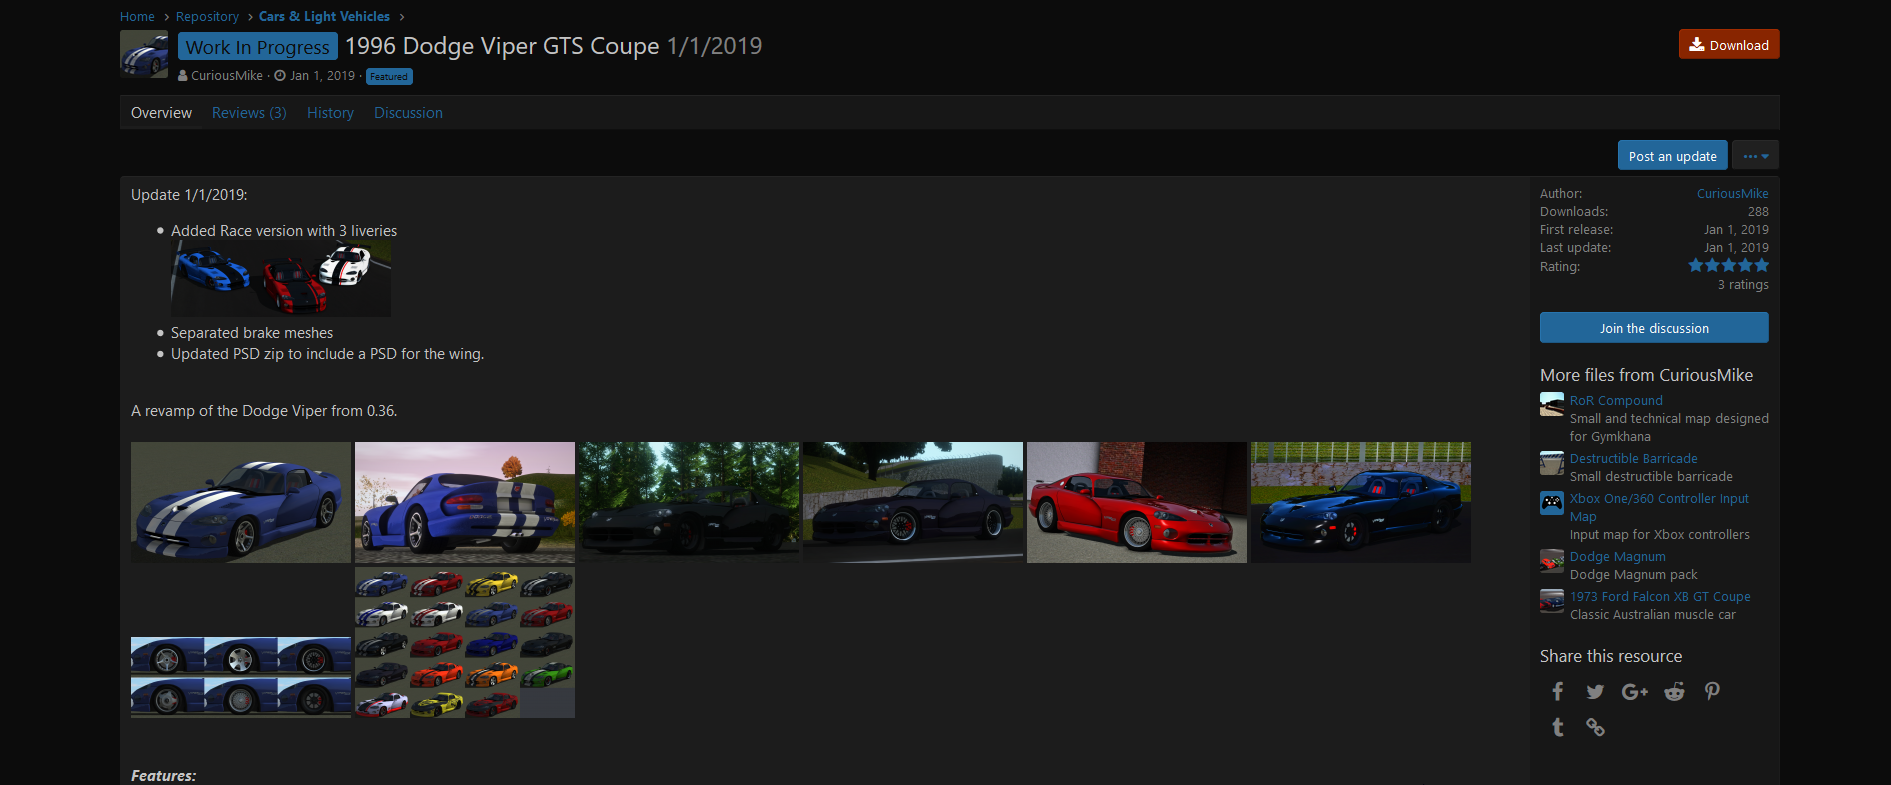
\includegraphics{images/repository-mod.png}

Click the \emph{Download} button at the top right of the page:

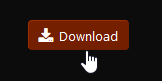
\includegraphics{images/repository-download.png}

\hypertarget{installing}{%
\subsection{Installing}\label{installing}}

Once the mod is downloaded, simply place the \texttt{*.zip} file into
\texttt{Documents\textbackslash{}Rigs\ of\ Rods\ 0.4\textbackslash{}mods}
or \texttt{\textasciitilde{}/.rigsofrods/mods} on Linux:

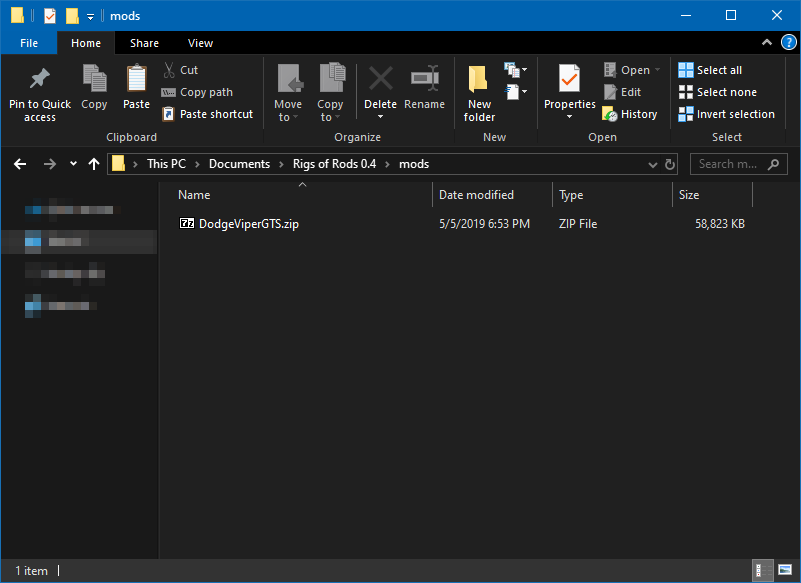
\includegraphics{images/repository-installing-mod.png}

\textbf{NEVER extract the zip file unless specifically mentioned in the
file description! I cannot stress this enough.}

You can organize your mods with subfolders.
(e.g.~\texttt{mods\textbackslash{}vehicles\textbackslash{}DodgeViperGTS.zip})

That's it! You can launch Rigs of Rods now and your shiny new mod should
be ready to use.

\hypertarget{installing-packs}{%
\section{Installing packs}\label{installing-packs}}

To install packs (a zip file containing multiple zips inside) such as
the
\href{http://forum.rigsofrods.org/resources/gabester-vehicle-pack.12/}{Gabester
Vehicle Pack} or the
\href{http://archives.rigsofrods.net/contentpacks/}{content packs}, just
extract the zip into the \texttt{mods} folder.

\hypertarget{installing-skinzips}{%
\section{Installing skinzips}\label{installing-skinzips}}

Some mods may provide a \texttt{*.skinzip} which contains some extra
liveries/skins for the vehicle. To install these, just place them inside
the \texttt{mods} folder.

For more information about skinzips, see
\href{/vehicle-creation/alternate-skins/}{this page}.

\hypertarget{psdpdn-files}{%
\section{PSD/PDN files}\label{psdpdn-files}}

These are files meant to be used by photo editing programs such as
Photoshop or paint.net, they are not meant to be placed in the RoR
directories.

%\hypertarget{aircraft-handling}{%
\chapter{Aircraft handling}\label{aircraft-handling}}

\hypertarget{how-to-use-the-autopilot}{%
\section{How to use the autopilot}\label{how-to-use-the-autopilot}}

You can find the autopilot on top of your dashboard in a plane. Upon
startup it looks like this:

The autopilot has different modes you can engage or disengage by
pressing the buttons. When you change a value, the change is immediately
applied to the current mode.

\hypertarget{heading-modes}{%
\subsection{Heading modes}\label{heading-modes}}

HDG (Heading): set the airplane heading to the heading selected (in
degree)

WLV (Wing Leveler): set the wings horizontal. The airplane should
roughly keep its current heading.

NAV (Radio Navigation): engage when approaching a runway equipped with
an ILS equipment (the red and white antennas). The airplane will first
try to intercept the runway axis, then stay along it until you pass the
runway edge.

\hypertarget{heading-listings}{%
\subsubsection{Heading Listings}\label{heading-listings}}

This is a list of headings to use for ILS on included maps.

North St.~Helens main runway - 240 degrees

Aspen main runway - 190 degrees

\hypertarget{altitude-modes}{%
\subsubsection{Altitude modes}\label{altitude-modes}}

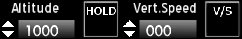
\includegraphics{images/autopilot-alt.jpg}

HOLD (Hold altitude): set the altitude to the altitude selected (in
feet). The the maximum vertical speed allowed to reach the altitude is
selected by the vert.speed setting (in feet per minute, the sign of the
selected vert speed is ignored). So this mode works better with a
vert.speed different than 0!

V/S (Vertical Speed): set the vertical speed (in feet per minute),
without a target altitude. Positive value to climb, negative to descent.

NAV+V/S (Vertical Radio Navigation): when both NAV and V/S are selected,
the altitude is controlled by the ILS system. So when approaching a
runway with NAV, engage V/S to make the plane descend to the runway.

\hypertarget{speed-mode}{%
\subsubsection{Speed mode}\label{speed-mode}}

ATHR (Auto-Throttles) set the speed of the airplane as selected in IAS
(Indicated Air Speed, in knots).

\hypertarget{other-buttons}{%
\subsubsection{other buttons}\label{other-buttons}}

GPWS (Ground Proximity Warning System): when engaged, a recorded voice
calls altitude and warns in case of dangerous maneuvers close to the
ground.

BRKS (Parking brakes)

\hypertarget{horizontal-navigation-indicator-hsi}{%
\subsection{Horizontal Navigation Indicator
(HSI)}\label{horizontal-navigation-indicator-hsi}}

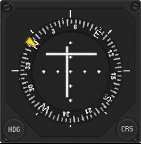
\includegraphics{images/autopilot-hsi.jpg}

There is a simplified HSI (Horizontal Navigation Indicator) instrument
between the AOA (Angle of Approach) indicator and the engine gauges. It
includes:

a compass

a heading bug (that runs along the heading selector)

two position indicators:

a vertical bar for horizontal deviation

a horizontal bar for vertical deviation.

They tell you how far you are from the optimal trajectory when you do an
ILS approach. The optimal position is when both bars are at the center
of the display.

\hypertarget{how-to-do-a-successful-instruments-approach-with-the-ils}{%
\subsection{How to do a successful instruments approach with the
ILS}\label{how-to-do-a-successful-instruments-approach-with-the-ils}}

ensure the approach you want to do is equipped with an ILS:

check if there are red and white antennas at the end of the runway, at
the side where you will touch down. Be sure the approach is clear of
obstacles.

fly to a comfortable distance from the runway, preferably off the
terrain.

ensure you are at the right altitude for an approach from that distance.
If the horizontal bar is low, descend, if it is high, climb.

fly in a way so you will soon intercept the runway axis, or are roughly
on the runway axis

Engage NAV, then V/S. Drop the joystick. The plane should fly by itself
now, intercepting the runway axis and descending to the runway.

You can see how it performs on the HSI display. The bars should cross at
the center when the approach is stabilized.

Control your speed! You should fly as slow as possible (around 100 knots
for the Antonov 12). Use auto-throttle if possible. Watch the AOA, if it
gets too high, you will stall! Add more flaps in that case.

If you go too fast, the plane will not descend and the horizontal bar
will go down.

On short final, the GPWS calls ``Minimums'': you reached the minimum
decision altitude. If you see the runway and everything is fine, proceed
to the landing (real pilots disconnect the autopilot at this stage and
land by the hand).

The autopilot should disconnect at the runway edge, but in some case it
can continue to function, so be cautious at the flare.

Engage reverses and brake (press and maintain key B). You landed!


\end{document}
